% Copyright (c) 2014,2016 Casper Ti. Vector
% Public domain.

\chapter{事件研究:2014年3月29日耀斑}\label{chap:3}
在这一章节中,我们主要讨论对2014年3月29日太阳上爆发的一个X1.1级耀斑色球辐射的辐射流体力学模拟的结果。我们利用RADYN和RH代码,基于拉马第高能太阳光谱成像探测器(\textit{Reuven Ramaty High Energy Solar Spectroscopic Imager,RHESSI}: \cites{Lin2002})卫星观测到的X射线功率谱数据对非热电子束参数的约束,对整个耀斑加热和冷却过程中的谱线形成和演化进行了比较深入的研究。这一部分与Mg \textsc{ii}谱线模拟有关的介绍、图片以及结果来自我即将发表的工作\textcites{Zhu2019}。


\section{耀斑事件与光谱观测简介}\label{sec:3}
世界时2014年3月29日17时48分在太阳活动区NOAA AR12017上爆发了一个大型的X1.1级耀斑,地面和空间的多个观测仪器都对这个耀斑进行了联合观测,包括太阳动力学观测台(\textit{Solar Dynamic Observtory, SDO}: \cites{Lemen2012}),RHESSI卫星,IRIS卫星,邓恩太阳望远镜(\textit{Dunn Solar Telescope, DST})等。在过去几年中对这个耀斑事件进行了大量的研究,在观测上,发现耀斑事件可能被一个暗条爆发事件触发\parencites{Kleint2015,Woods2018},大约有$3\times10^{30}\ \mathrm{erg}$的磁场自由能在耀斑中释放\parencites{Aschwanden2015},并以非热电子和热传导的形式加热低层大气\parencites{Battaglia2015}。部分重联加速的非热电子轰击环顶产生终止激波\parencites{Polito2018}并加速更多电子沿环向下传播。随着低层大气的加热,出现了环状的耀斑带\parencites{LiuC2015}。在耀斑带上可以观测到强烈的Balmer连续谱增强\parencites{Heinzel2014},UV谱线增强\parencites{Liu2015}和色球蒸发\parencites{Young2015,Li2015}。进一步地,还能观测到这次耀斑事件产生的日震\parencites{Judge2014}。

之前的辐射流体力学模拟也对这个耀斑产生的色球谱线进行了一定的研究,\textcites{Rubio2016}利用RADYN和RH代码对这个耀斑进行了模拟,她们同样使用了基于RHESSI卫星观测的随时间演化的非热电子参数,总体能流大约在$10^{11}-10^{12}\ \mathrm{erg\  s^{-1}}$之间变化。基于此她们计算了H$\alpha$,Ca \textsc{ii}和Mg \textsc{ii}等一系列色球谱线在加热过程中的谱线形状。对于Mg \textsc{ii}线她们发现在自洽的模拟大气中很难再现谱线非线心反转的谱线,需要人工提高过渡区下线心形成高度的电子密度才有可能得到这样的谱线。\textcites{Kowalski2017a}同样对这个耀斑进行了基于RADYH代码的数值模拟,他们采用了两个较高的电子束能流输入,能流最大值分别为$10^{11}\ \mathrm{erg\  s^{-1}}$(以下记作F11)和$5\times10^{11}\ \mathrm{erg\  s^{-1}}$(以下记作5F11),并较好的再现了Fe \textsc{ii}谱线在耀斑带上的形状。
\section{模拟输入设定}
我们在这一部分中同样将利用RADYN代码和RH代码来模拟2014年3月29日耀斑中色球UV谱线的随时间演化。首先我们利用RADYN代码获得太阳大气在被非热电子束加热后随时间演化的结果,再利用RH代码精细地计算这些UV谱线轮廓随时间的演化。对于RADYN代码,我们将利用和\textcites{Kowalski2017a}中相同的初始大气设置和电子束输入。对一维初始大气而言,我们使用了一个半圆形长为10 Mm的耀斑环大气,在环的顶点,电子密度为$8\times10^9\ \mathrm{cm^{-3}}$,温度为3.2 MK。对于加热电子束的参数,我们使用了$E_c=25$ KeV,$\delta = 4.2$,电子束的能流采用了5F11模型,且在模拟中上下变化。

在RH代码的设置中,我们使用了STARK-B数据库中对Mg \textsc{ii}谱线的Stark致宽数据来计算这一系列谱线的在给定一维大气中的辐射转移过程。为了和IRIS观测相比较,我们计算了了方向角$\mu = 0.77$的辐射转移得到的谱线轮廓。对于各条研究的谱线,我们都将对应的原子在代码中设为\texttt{active}模式,即能够完全求解NLTE下的辐射转移和能级粒子数。同时我们还计算了一个六能级的氢原子模型在NLTE下的辐射转移来提供诸如Balmer连续谱、Paschen连续谱和一系列Balmer系线对整个光谱能量分布(\textit{spectral energy distribution, SED})函数的影响。
\section{大气演化过程}
\begin{figure}
	\centering
	\includegraphics[width=0.8\textwidth]{figs/5F11_atmos_rev}
	\caption{5F11模型中的耀斑带上大气电子密度$n_e$、温度$T$和一维速度$v_z$随时间变化图。不同颜色的曲线代表模拟中的不同时刻。}
	\label{fig:3.1}
\end{figure}
我们在这一部分讨论RADYN代码得到的耀斑大气演化模型。图~\ref{fig:3.1}展示了电子密度$n_e$、温度$T$和一维速度$v_z$在模拟中的不同时刻在不同高度上的分布。可以看到整个大气结构随着非热电子束的不断加热发生了剧烈的变化,包含温度的上升、高色球的加热与剧烈的色球蒸发与凝聚过程。

在$t=2.6$ s时,高色球已经被剧烈加热至$3\times 10^4$ K。此时大气中的中性氢已经基本被完全电离,大气中的电子密度相比于初始大气已经上升了1-3个量级。在低日冕中约为1.25 Mm处,一个速度约为200 $\mathrm{km\  s^{-1}}$的色球蒸发过程已经出现。同时还伴随着过渡区和色球区域一个大约为20 $\mathrm{km\  s^{-1}}$的物质下流。由于色球顶部的加热,过渡区已经向下移动了大约25 km。

在$t=6.3$ s时,物质下流的体速度(\textit{bulk velocity})已经达到了约150 $\mathrm{km\  s^{-1}}$,且整个下流物质有大约100 km高。物质的向下流动拉伸的过渡区的高度,使其温度梯度减小。同时可以看到在日冕中有一团温度较低、电子密度较大的物质在向上传播。

在$t=7.35$ s时,下流物质逐渐到达较低的色球。由于色球密度远远高于过渡区密度,粒子的碰撞等一系列过程逐渐使得下流的体速度开始逐渐减小。之前被拉伸的过渡区位置又重新被压缩。同时这些相互作用也在过渡区下形成了一些电子密度较大$\sim 10^{14}\ \mathrm{cm}^{-3}$,但温度较低$\sim 1-2\times 10^{4}$ K的“团块”。这些团块在之后的时间内(如$t=8.28$ s)又逐渐随着过渡区的下移(物质的不断被加热)而并合在一起。

在$t=10$ s后,物质下流速度从40 $\mathrm{km\  s^{-1}}$继续减小,过渡区继续降低并压缩色球。相比于之前比较复杂的大气结构,整个大气变得趋于平静。在过渡区下方,形成了一个电子密度的高峰,达到了$5\times10^{14}-10^{15}\ \mathrm{cm^{-3}}$,接近\textcites{Rubio2017}中通过人工提高大气中的电子密度来实现Mg \textsc{ii}线的非线心反转的电子密度。

\begin{figure}
	\centering
	\includegraphics[width=\textwidth]{figs/MgII_SB}
	\caption{模拟中$t=23.53$ s时的Mg \textsc{ii}谱线轮廓与IRIS卫星观测的比较。黄色谱线轮廓代表未修改的RH代码得到的结果,蓝色谱线轮廓代表IRIS观测,上图中的粉色谱线代表RH+SB得到的结果,下图中的粉色谱线代表RH+SB$\times$30得到的谱线轮廓。经过辐射定标(\textit{radiometric calibration})后的IRIS观测数据被乘上了一个36的因子来获得与RH合成光谱相近的辐射强度。这个填充因子(\textit{filling factor})可能来自于IRIS观测的分辨率限制。}\label{fig:3.2}
\end{figure}

\section{谱线演化:Mg \textsc{ii}}\label{sec:3.4}
在这一部分中我们将讨论Mg \textsc{ii}谱线轮廓在模拟中的演化以及和IRIS观测到的耀斑带上的谱线轮廓的对比。对于Mg \textsc{ii} h和k线而言,在大的耀斑带上能够观测到两种特征的谱线轮廓,一种是带有很强的红翼不对称性,另一种是比较对称,无线心反转且线翼剧烈增宽的谱线\parencites{Panos2018}。我们这里主要尝试再现第二种谱线,对前者我们仅对其可能出现的原因进行简单的讨论。在具体模拟中,我们使用了一个10能级的Mg \textsc{ii}原子模型,包含Mg \textsc{ii}基态(Mg \textsc{i}连续态)和连续态(Mg \textsc{iii}基态)来计算辐射转移。

在图~\ref{fig:3.2}中,我们展示了$t=23.53$ s时合成(\textit{synthetic})的Mg \textsc{ii}谱线轮廓和IRIS观测的比较。可以看到RH代码比较好地再现了Mg \textsc{ii}线非线心反转的谱线特征,且使用STARK-B数据库后的RH代码(以下记为RH+SB)给出了比原有RH代码更加宽且增强的线翼辐射,但相比于IRIS观测(蓝线)中剧烈的线翼增强还是有比较大的差距。针对这一点,我们进行了一个大胆的尝试,我们直接在STARK-B数据库中所有Mg \textsc{ii}谱线的$\Gamma_{stark}$上乘了一个30的因子(以下记作RH+SB$\times$30)。在这样的处理之后,我们能够获得了和观测拟合的非常好的谱线轮廓,预示着Mg \textsc{ii}线间的连续谱辐射增强可能来自于这些谱线剧烈增强的线翼辐射。

\begin{figure}
	\centering
	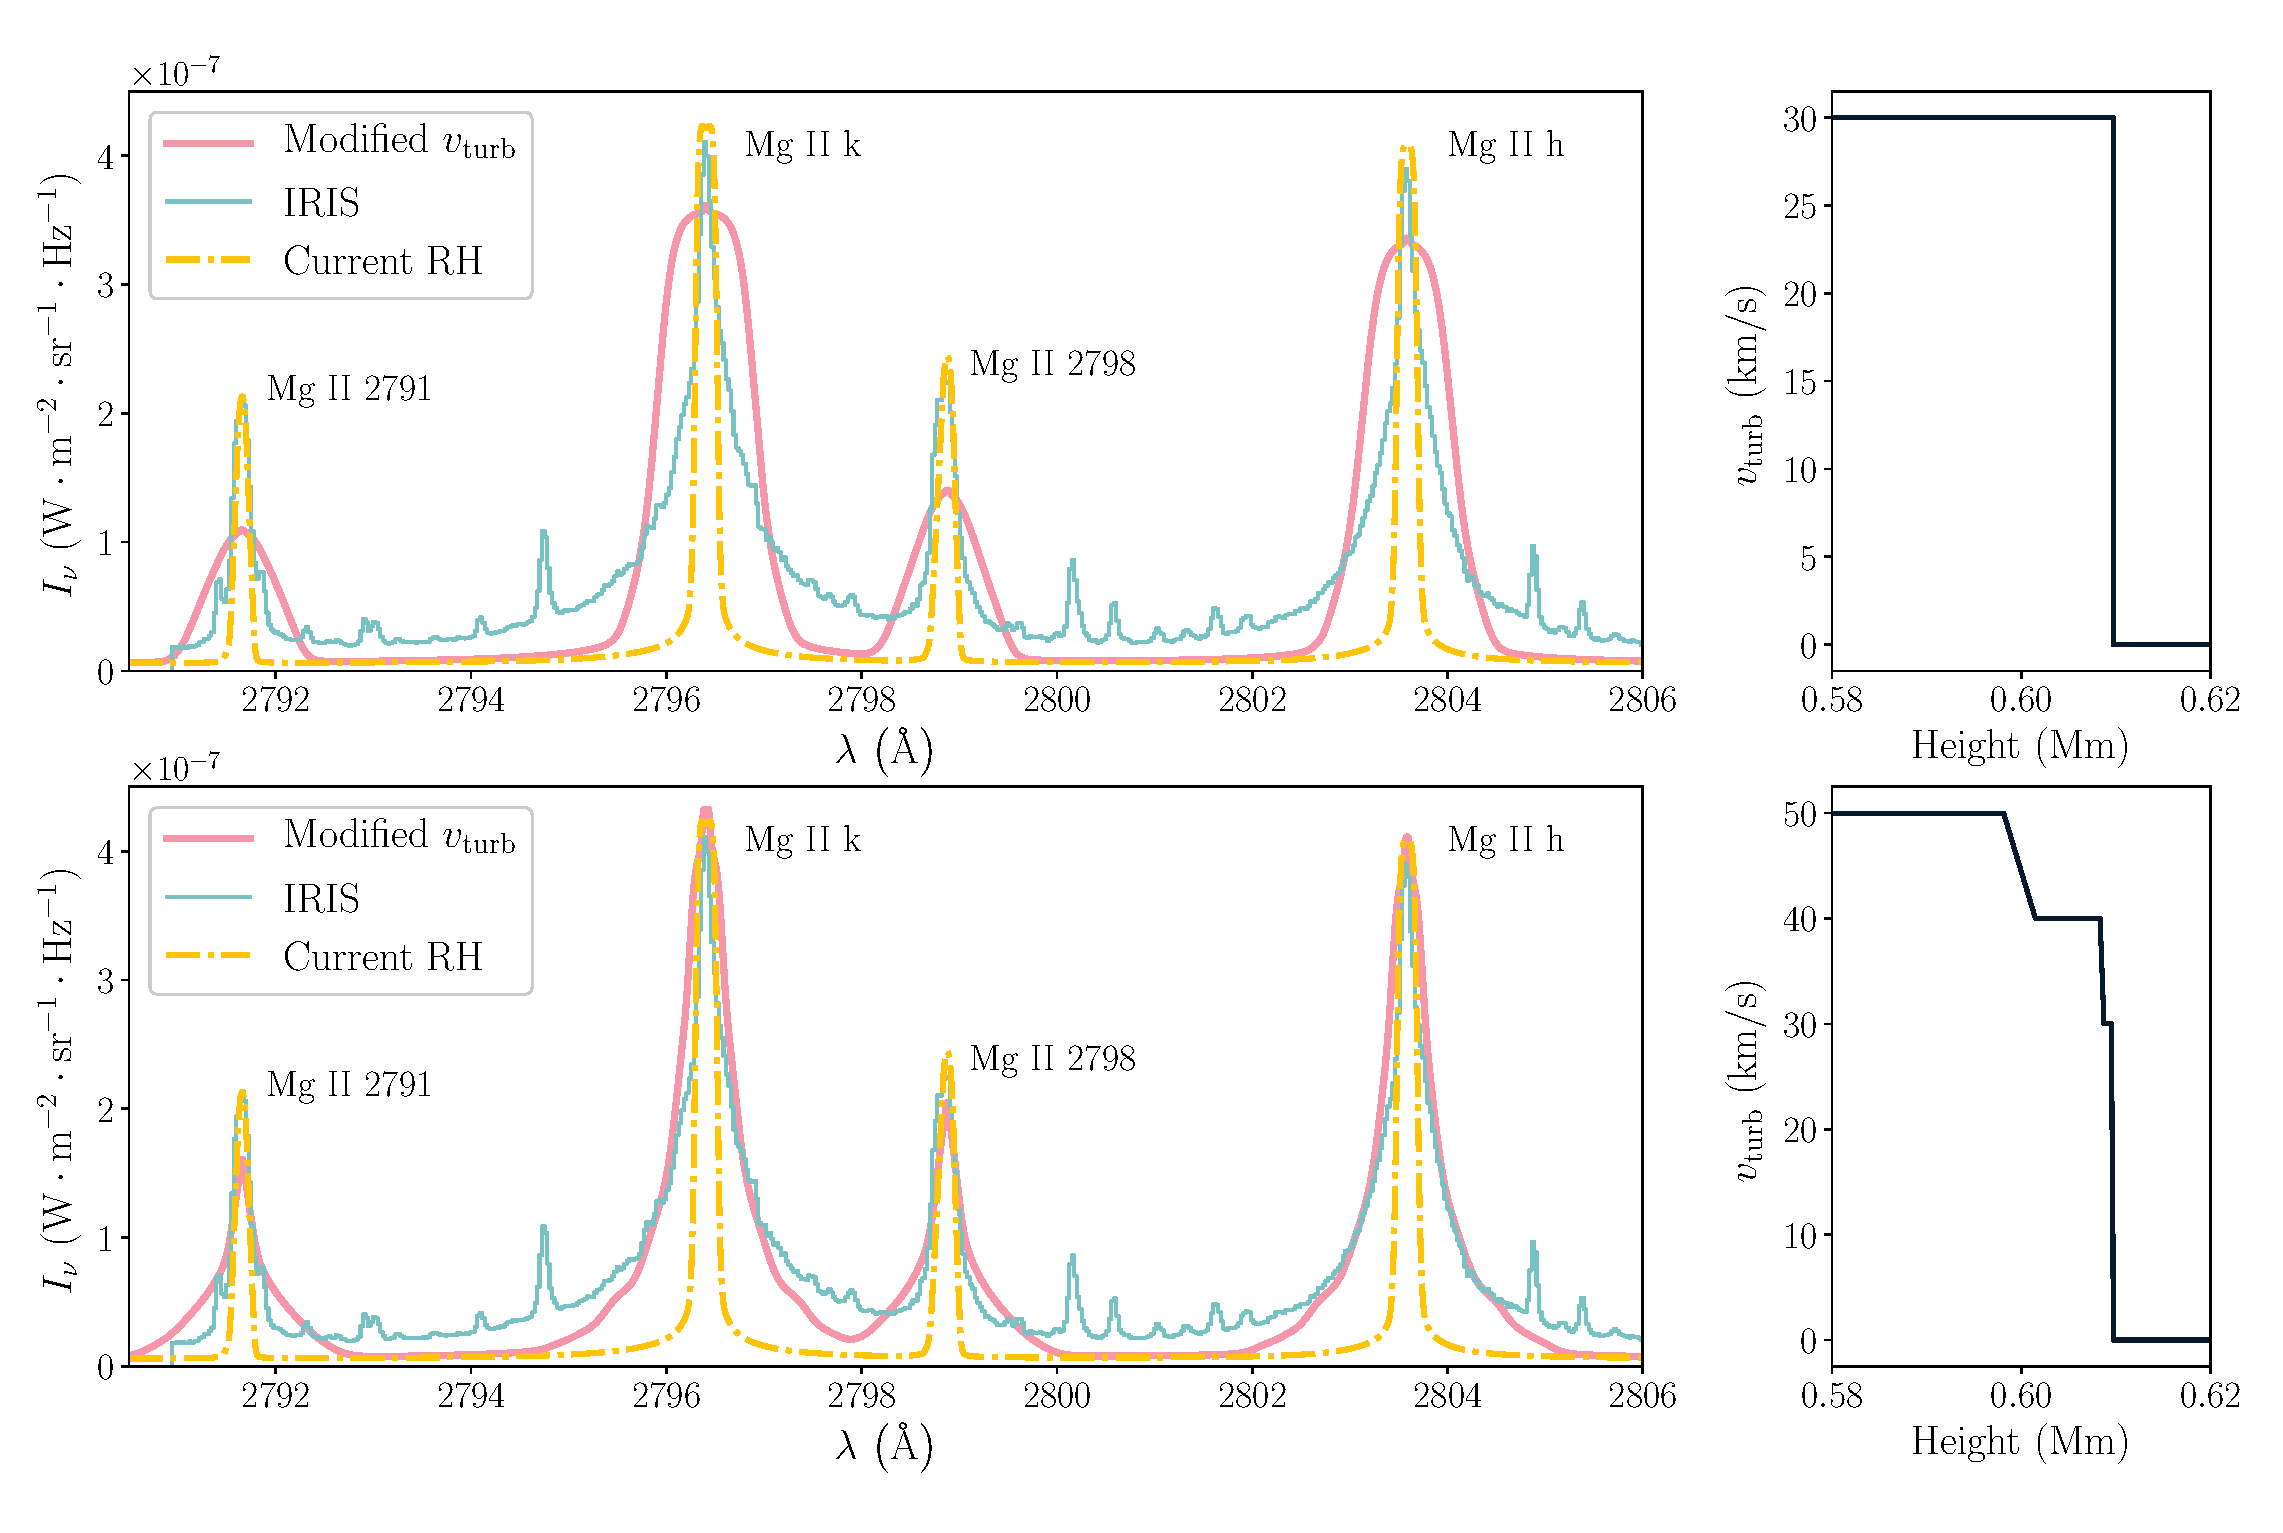
\includegraphics[width=\textwidth]{figs/MgII_vturb}
	\caption{通过调节大气中的微湍动速度分布来实现Mg \textsc{ii}谱线的致宽。上图粉色轮廓来自恒定的$30\ \mathrm{km \  s^{-1}}$的湍动速度的耀斑大气,下图粉色轮廓来自湍动速度从线心形成高度逐渐增加到$50\ \mathrm{km \  s^{-1}}$的耀斑大气。}\label{fig:3.3}
\end{figure}

为了排除诸如微湍动速度等因素对谱线致宽的影响,我们尝试人工调节RADYN输出大气中的湍动速度在不同高度的分布来观察Mg \textsc{ii}谱线的轮廓变化。我们在同图~\ref{fig:3.2}中相同时刻的大气中插入了两种湍动速度的分布,一种是恒定的$30\ \mathrm{km \  s^{-1}}$的湍动速度(图~\ref{fig:3.3}上半图),另一种是从线心形成高度逐渐增加到$50\ \mathrm{km \  s^{-1}}$(图~\ref{fig:3.3}下半图)。从图~\ref{fig:3.3}中可以看出对于前者来说,由于在RH代码中湍动速度的分布是Gaussian形的,因此过大的湍动速度直接导致了整个谱线的形状都被Gaussian形的谱线所主导,这样的谱线轮廓在线心处太宽,且在线翼处增强不大,因此不能较好的再现谱线的致宽。而对于后者而言,虽然我们能够通过从线心开始逐渐增加湍动速度来达到使Mg \textsc{ii} h和k线轮廓与观测符合的比较好的结果,但是由于Mg \textsc{ii}三重线和Mg \textsc{ii} h,k两线在此时的形成高度相近,导致了合成的Mg \textsc{ii}三重线相比于观测到的谱线轮廓更加宽了。因此我们认为提高微湍动速度并不是解释谱线剧烈致宽的主要机制。

\begin{figure}
	\centering
	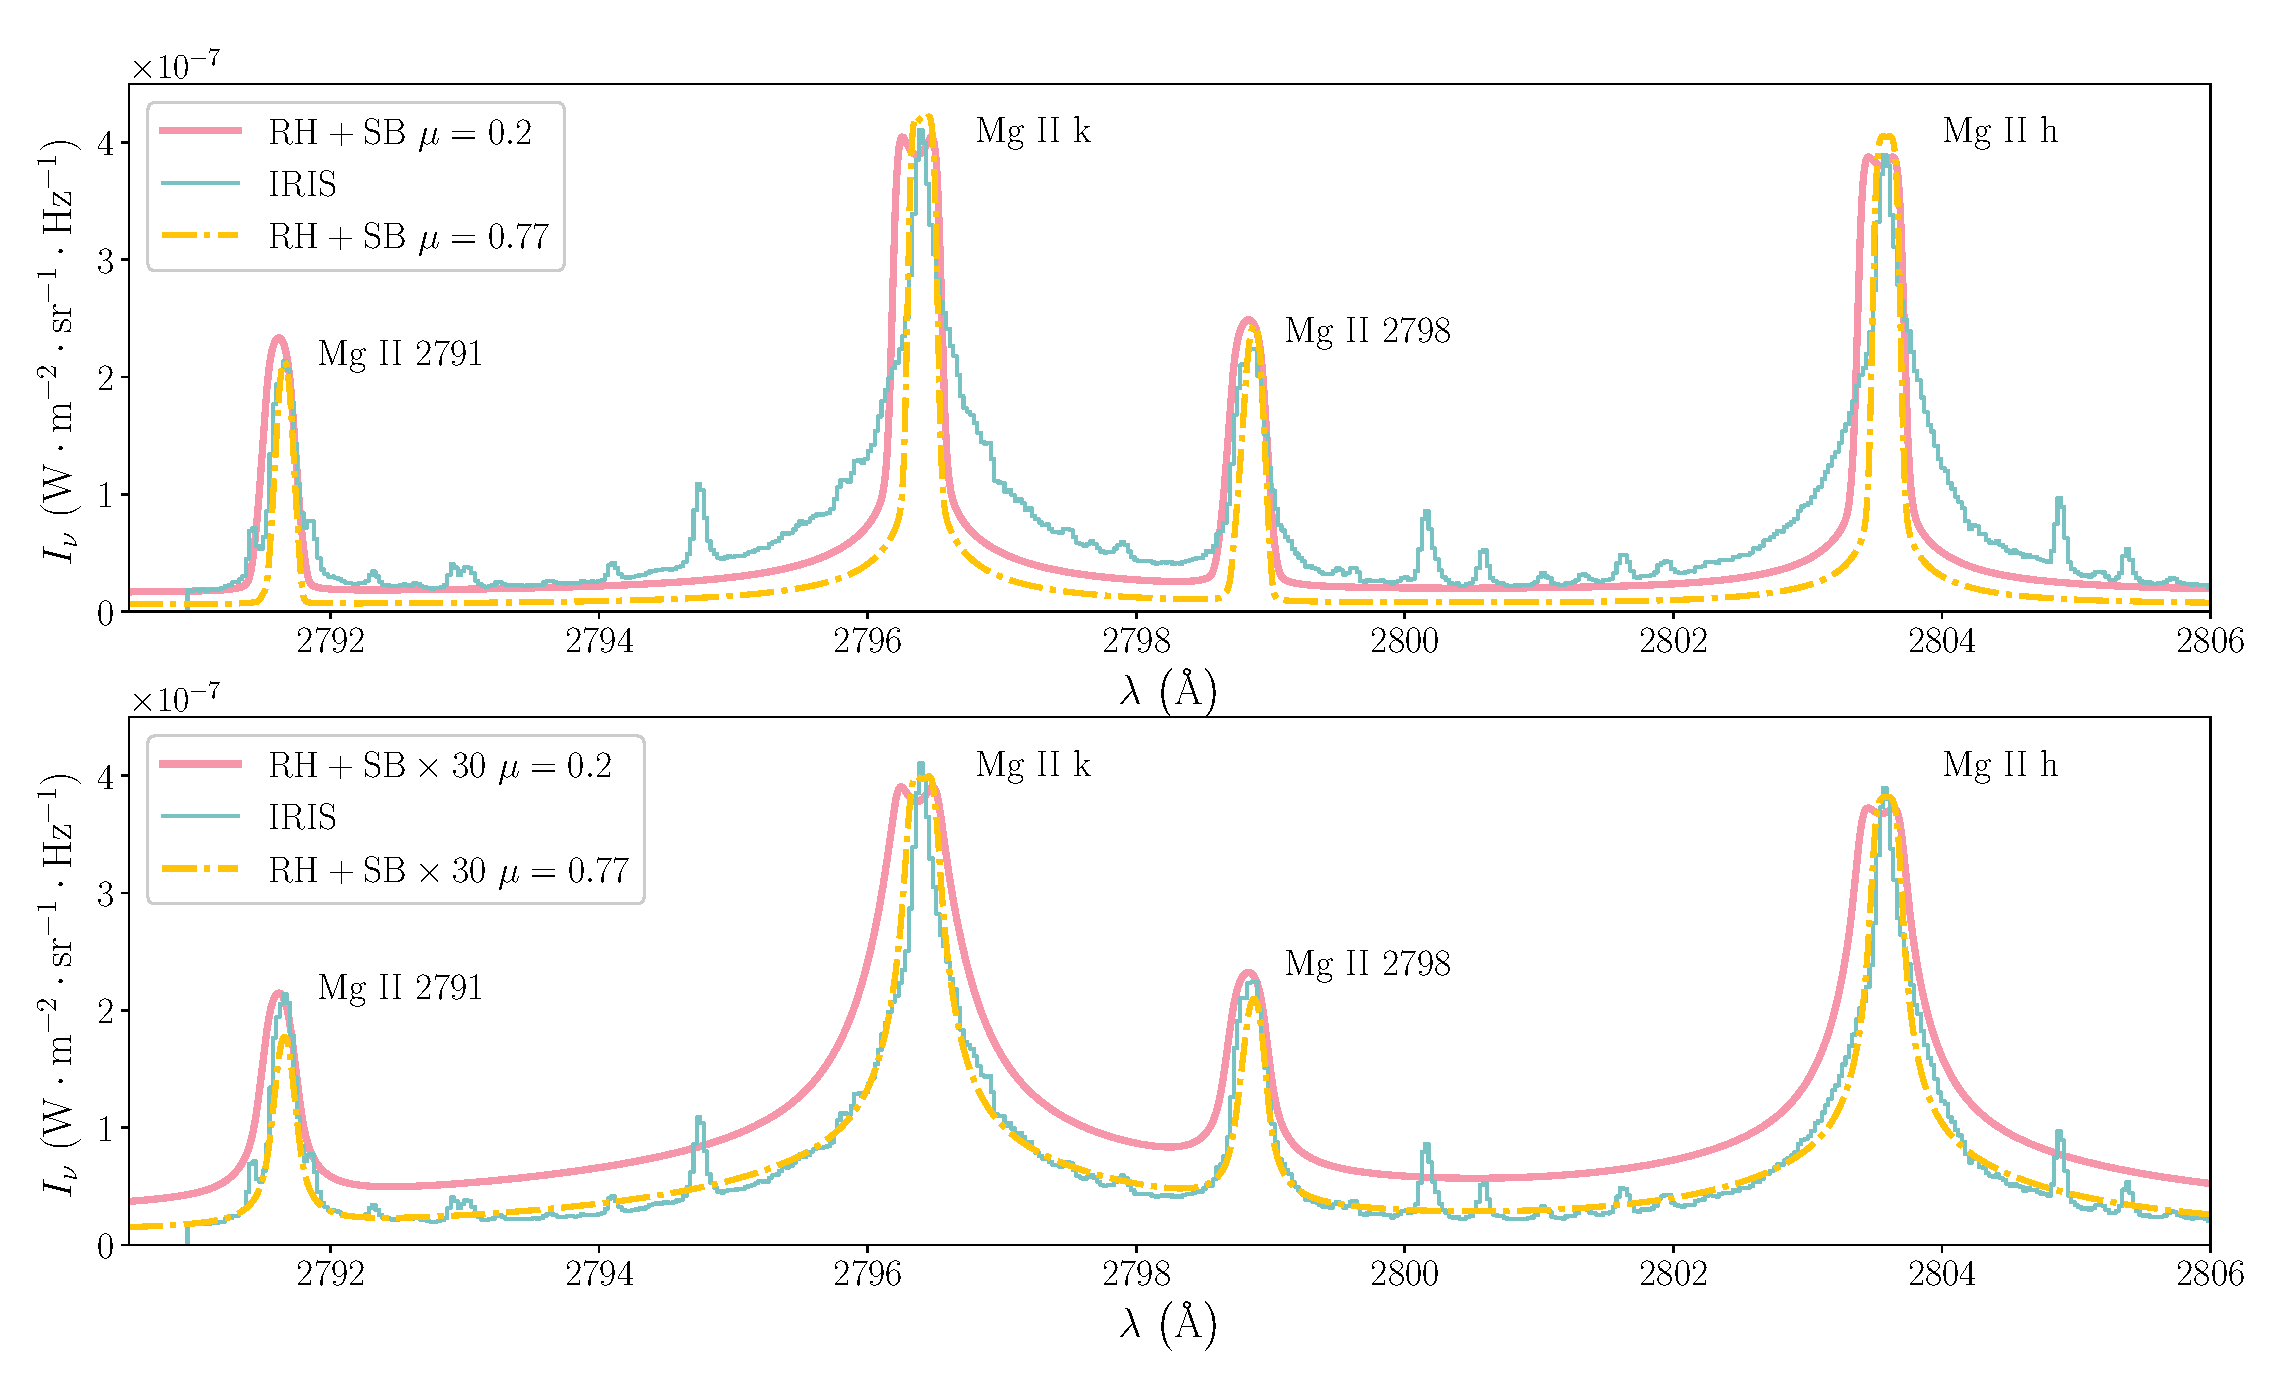
\includegraphics[width=\textwidth]{figs/MgII_mu02}
	\caption{模拟中$t=23.53$ s时在不同方向角$mu$下计算的合成Mg \textsc{ii}谱线轮廓与IRIS卫星观测的比较。上半图为RH+SB中$\mu=0.2$(粉色实线)和$\mu = 0.77$(黄色点划线)下的合成谱线轮廓。下半图为为RH+SB$\times$30中$\mu=0.2$(粉色实线)和$\mu = 0.77$(黄色点划线)下的合成谱线轮廓。}
	\label{fig:3.3.5}
\end{figure}

最后,我们还讨论了视线方向角$\mu$对Mg \textsc{ii}谱线轮廓的影响。在图~\ref{fig:3.3.5}中我们比较了在RH+SB和RH+SB$\times$30中$\mu=0.2$和$\mu=0.77$。$\mu$越小,说明视线方向和平面平行层大气的法线方向夹角越大(对太阳观测而言越靠近临边)。$\mu = 0.2$的谱线轮廓与$\mu = 0.77$的谱线轮廓相比,线翼辐射更强,红移越小(投影速度小),且谱线线心反转越明显。这一现象的简单解释可以参见\ref{sec:3.7}节。

\begin{figure}[htbp]
	\begin{minipage}[t]{0.48\linewidth}
	\centering
	\includegraphics[width=0.95\linewidth]{figs/5F11_spectra_1_mg}
	\end{minipage}%
	\hfill
	\begin{minipage}[t]{0.48\linewidth}
	\centering
	\includegraphics[width=0.95\linewidth]{figs/5F11_spectra_2_mg}
	\end{minipage}
	\caption{RH+SB(左)和RH+SB$\times30$(右)下的Mg \textsc{ii}合成谱线轮廓演化。为了能够清楚地显示不同时刻的轮廓,不同时刻的谱线轮廓被人为向上移动了一段距离。}
	\label{fig:3.4}
\end{figure}


基于以上的研究,我们分别在RH+SB和RH+SB$\times30$下计算了Mg \textsc{ii}各条谱线在整个演化过程中的轮廓(图~\ref{fig:3.4})。在$t=2.6$ s和$t=6.3$ s,由于低层大气已经被非热电子束剧烈加热,Mg \textsc{ii}各条线的辐射强度均有剧烈增强。两套计算方法中此时的谱线轮廓仍存在线心反转,同样来自于在线心形成高度源函数和Planck函数的脱耦\parencites{Rubio2016}。

在$t=7.35$ s时,Mg \textsc{ii} h,k和三重线都明显增宽,这主要来自于此时速度上流和下流中都对Mg \textsc{ii}谱线形成有所贡献导致的两个不同Doppler频移的分量的叠加。在RH+SB$\times30$中有更多的光子因为Stark致宽而被散射到线翼上,因此相比于RH+SB的结果,其线心反转反而不再明显。

在$t=8.28$ s时,所有的Mg \textsc{ii}线都出现了一个静止分量和一个红移分量,这个红移分量来自于速度下流部分物质对Mg \textsc{ii}线辐射的贡献。这些谱线在观测中都不太常见,但我们猜测耀斑带前缘的红翼不对称的Mg \textsc{ii}谱线可能来自于这些红移分量的叠加效应,之前\textcites{Rubio2016}的多环(\textit{multi-thread})的模拟也指出了这一点。

在$t=10$ s后,Mg \textsc{ii}线的红移随着速度下流的逐渐减小而减小。此时Mg \textsc{ii}的线心形成高度正好处于过渡区下的高电子密度区域(详细分析见\ref{sec:3.7}节),较高的电子密度维持了一个近似于LTE的环境,使得线心源函数与Planck函数的脱耦并不明显,线心反转消失。由于Stark致宽效应主要发生在线翼区域,因此其仅仅产生了更加增强的线翼辐射。

\section{谱线演化:C \textsc{ii}}

\begin{figure}
	\centering
	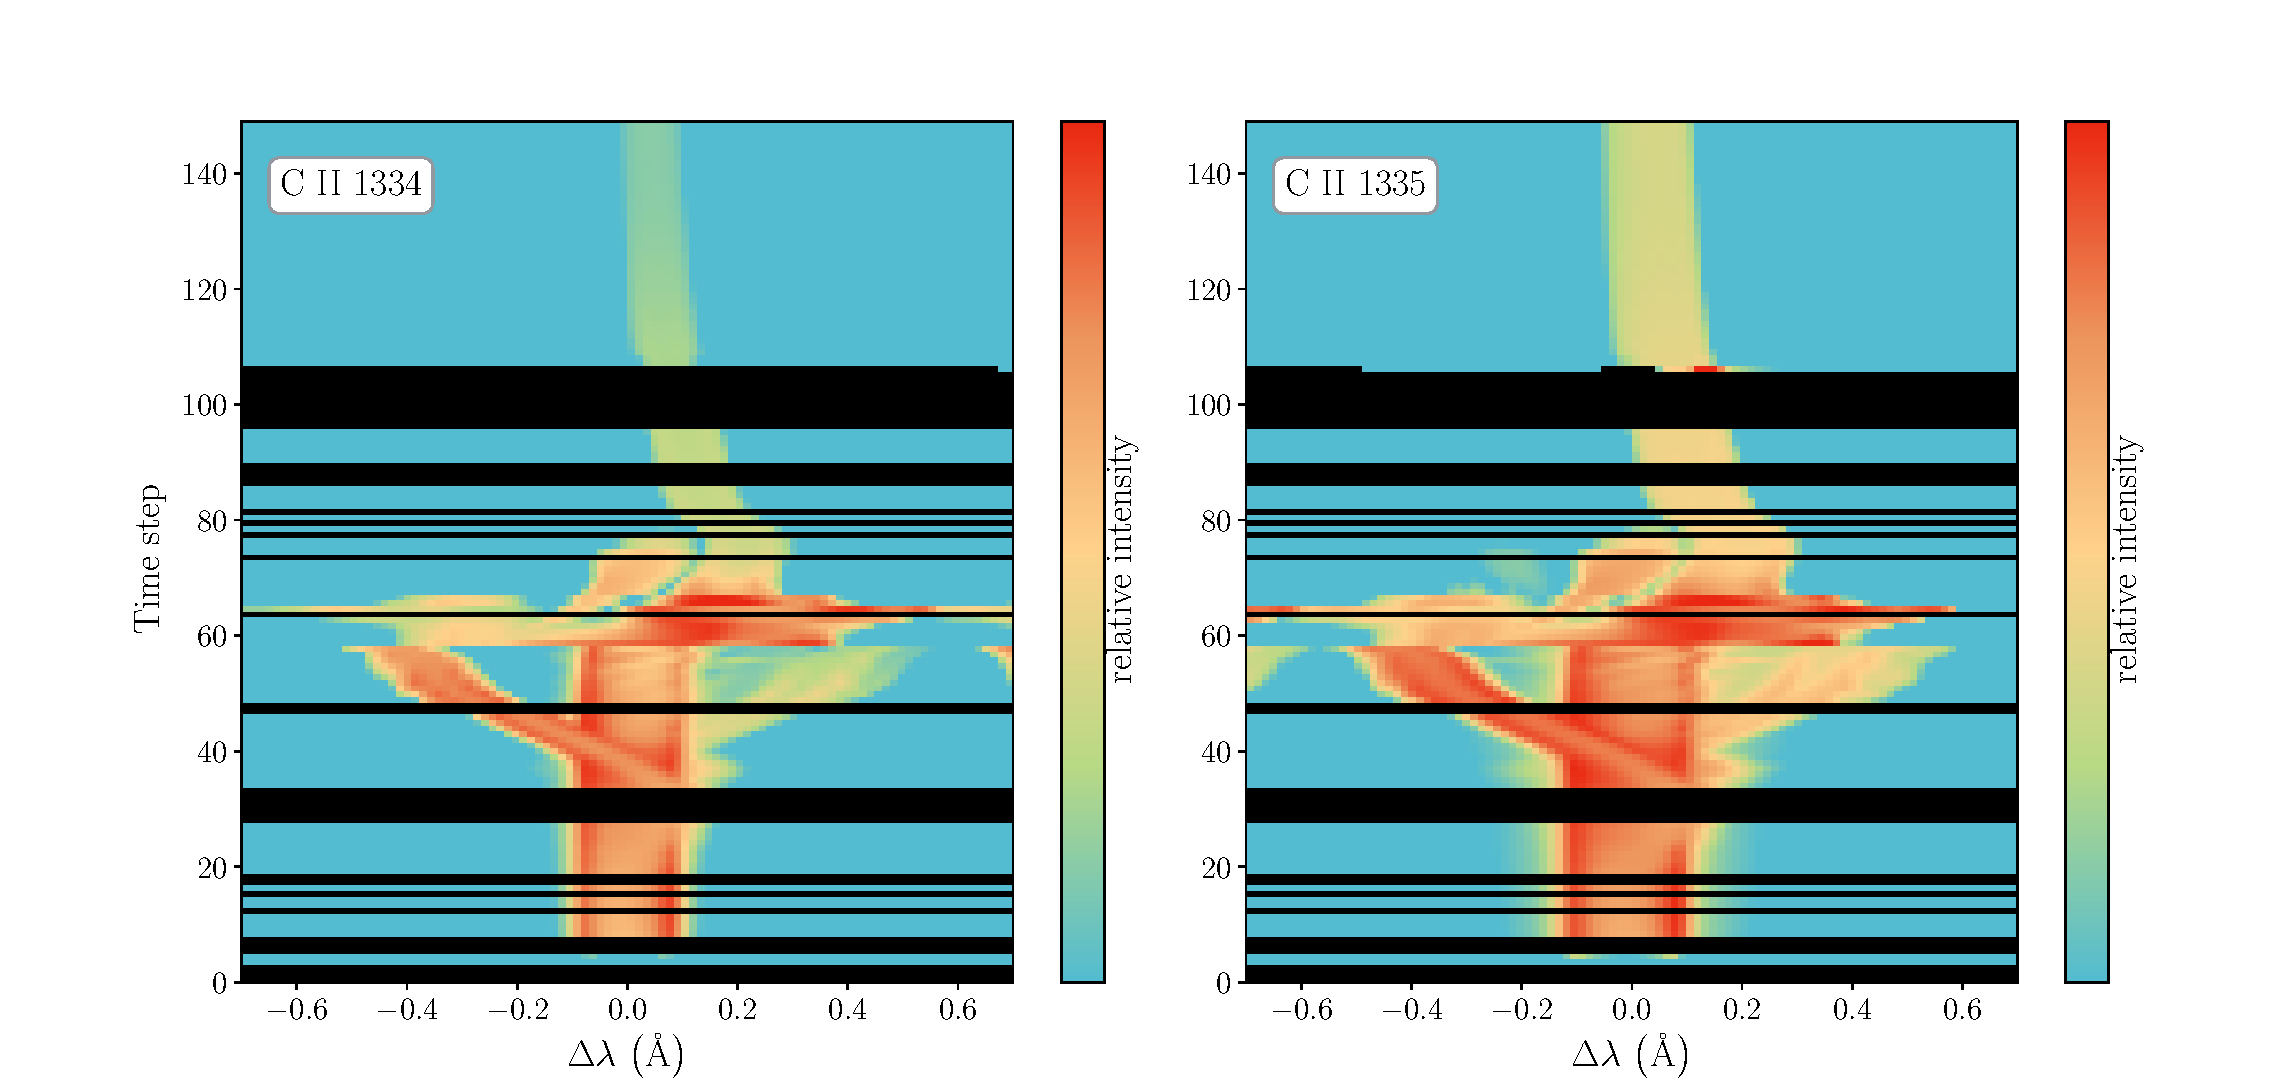
\includegraphics[width=\textwidth]{figs/5F11_spectra_imshow_C}
	\caption{C \textsc{ii}双重线强度随时间演化图,横坐标为波长,纵坐标为不同时刻,颜色代表该波长和时刻下的辐射强度。图中黑色部分为为由于数值原因无法收敛或者出现运算崩溃的时刻。}
	\label{fig:3.5}
\end{figure}

在这一部分我们将讨论基于同样的RADYN耀斑大气演化所计算的C \textsc{ii}双重线的谱线轮廓演化。此处我们使用了RH代码自带的一个9能级的C \textsc{i}和C \textsc{ii}原子模型,包含C \textsc{i}的三个能级和6个C \textsc{ii}的能级。图~\ref{fig:3.5}展示了这两条线在所有能够正确计算的时刻其谱线内的辐射强度随着时间的演化。图中的黑色区域为由于数值原因无法收敛或者出现运算崩溃的时刻。同时我们还挑选了一些计算收敛且有代表性的谱线轮廓展示在图~\ref{fig:3.6}中。这些时刻的问题可能来自于在高温度时计算碰撞电离时的LU分解出现奇异性。
\begin{figure}
	\centering
	\includegraphics[width=\textwidth]{figs/5F11_spectra_line_C}
	\caption{和图~\ref{fig:3.1}中时刻相近大气中计算得到的C \textsc{ii}双重线谱线轮廓。}
	\label{fig:3.6}
\end{figure}


总体上来说,我们可以大致描述整个C \textsc{ii}线的轮廓随时间演化的大致趋势。在前2 s左右,整个谱线还处在线心反转的大致形状中(图~\ref{fig:3.6}中$t=2.6$ s的粉色轮廓)。在$2-4$ s间,原来线心反转中的蓝翼峰不断增强,红翼峰不断减弱,形成了一个有明显蓝翼增强的谱线。之后在$t=6 s$左右随着色球凝聚的出现以及一个向上运动冷且密度较大的物质流的出现,C \textsc{ii}谱线出现了一个蓝移分量和一个红移分量(如$t=6.3$ s时的红色轮廓)。在$t=7$ s左右,物质下流的速度达到最大,C \textsc{ii}谱线出现了剧烈的红翼不对称性(图~\ref{fig:3.6}中黄色轮廓)。在$t=8$ s后谱线强度逐渐减弱,和Mg \textsc{ii}线类似出现了一个静止分量和一个红移分量(推测来自于两条线形成高度随着色球压缩而不断靠近)。之后的谱线轮廓演化也和Mg \textsc{ii}线类似,在$t=10$ s后静止分量基本消失,谱线红移逐渐减小,发射强度也随之降低(图~\ref{fig:3.6}中)。由于存在着另一条谱线的重叠,C \textsc{ii} 1335 \mbox{\AA}线的轮廓和1334 \mbox{\AA}的轮廓略有不同,谱线内积分强度较大,但是没有本质上的区别。

由于之前在图~\ref{fig:3.2}中$t=23.53$ s的Mg \textsc{ii}谱线轮廓在RH+SB$\times30$中的计算与观测取得了比较好的结果,我们同样比较了同一时间的合成光谱中的C \textsc{ii}双重线轮廓与耀斑带上同一地点同一时间的C \textsc{ii}线观测轮廓(图~\ref{fig:3.7})。我们发现尽管合成光谱中Mg \textsc{ii}线的Doppler频移能够和具体观测得到比较好的拟合,但是合成的C \textsc{ii}线与实际观测到的C \textsc{ii}线红移不太相符。即我们没有办法在模拟中同时比较好地再现C \textsc{ii}线和Mg \textsc{ii}线轮廓。在利用C \textsc{i} 1354.288 \mbox{\AA}线对FUVS部分的谱线进行严格的波长定标之后,我们发现如图~\ref{fig:3.7}上半图中粉色轮廓所示,其线心位置和IRIS观测到的线心大约相距$\sim 0.062$ \mbox{\AA},折合约为$\sim 14\ \mathrm{km\  s^{-1}}$。在模拟当中红移和观测大致相符的谱线大约出现在$t=13.0$ s左右(图~\ref{fig:3.7}中黄色点划轮廓)。

由于STARK-B数据库中并没有这C \textsc{ii}这几条谱线的Stark致宽数据,但是从图~\ref{fig:3.7}上半图中可以明显看出谱线在远线翼致宽仍然远远不足。受之前的Mg \textsc{ii}线的调整启发,我们直接在RH代码中人工调整$\Gamma_{Stark}$。我们发现,如果要让$t=23.53$ s和$t=13.0$ s的红侧远线翼产生足够的辐射增强,需要在$t=23.53$ s的$\Gamma_{Stark}$乘上一个约为740的因子,或者在$t=13.0$ s的谱线的$\Gamma_{Stark}$上乘上一个290的因子。此外,我们的谱线尚不能很好的再现在蓝翼的一些辐射增强。

\begin{figure}
	\centering
	\includegraphics[width=\textwidth]{figs/5F11_IRIS_CII}
	\caption{合成的C \textsc{ii}双重线与IRIS观测的比较。上半图中展示了RH代码输出中$t=23.53$ s和$t=13.0$ s的谱线轮廓和IRIS观测的对比,下半图展示了通过人工增加Stark致宽和移动波长得到的$t=23.53$ s的谱线轮廓、仅增加Stark致宽得到的$t=13.0$ s的谱线轮廓和IRIS观测的对比。其中竖线代表了三条C \textsc{ii}线的真空静止波长。其中的IRIS观测经过辐射定标之后同样乘了一个10的因子使其强度与RH合成光谱可比。}
	\label{fig:3.7}
\end{figure}

\section{谱线演化:Si \textsc{iv}}
\begin{figure}
	\centering
	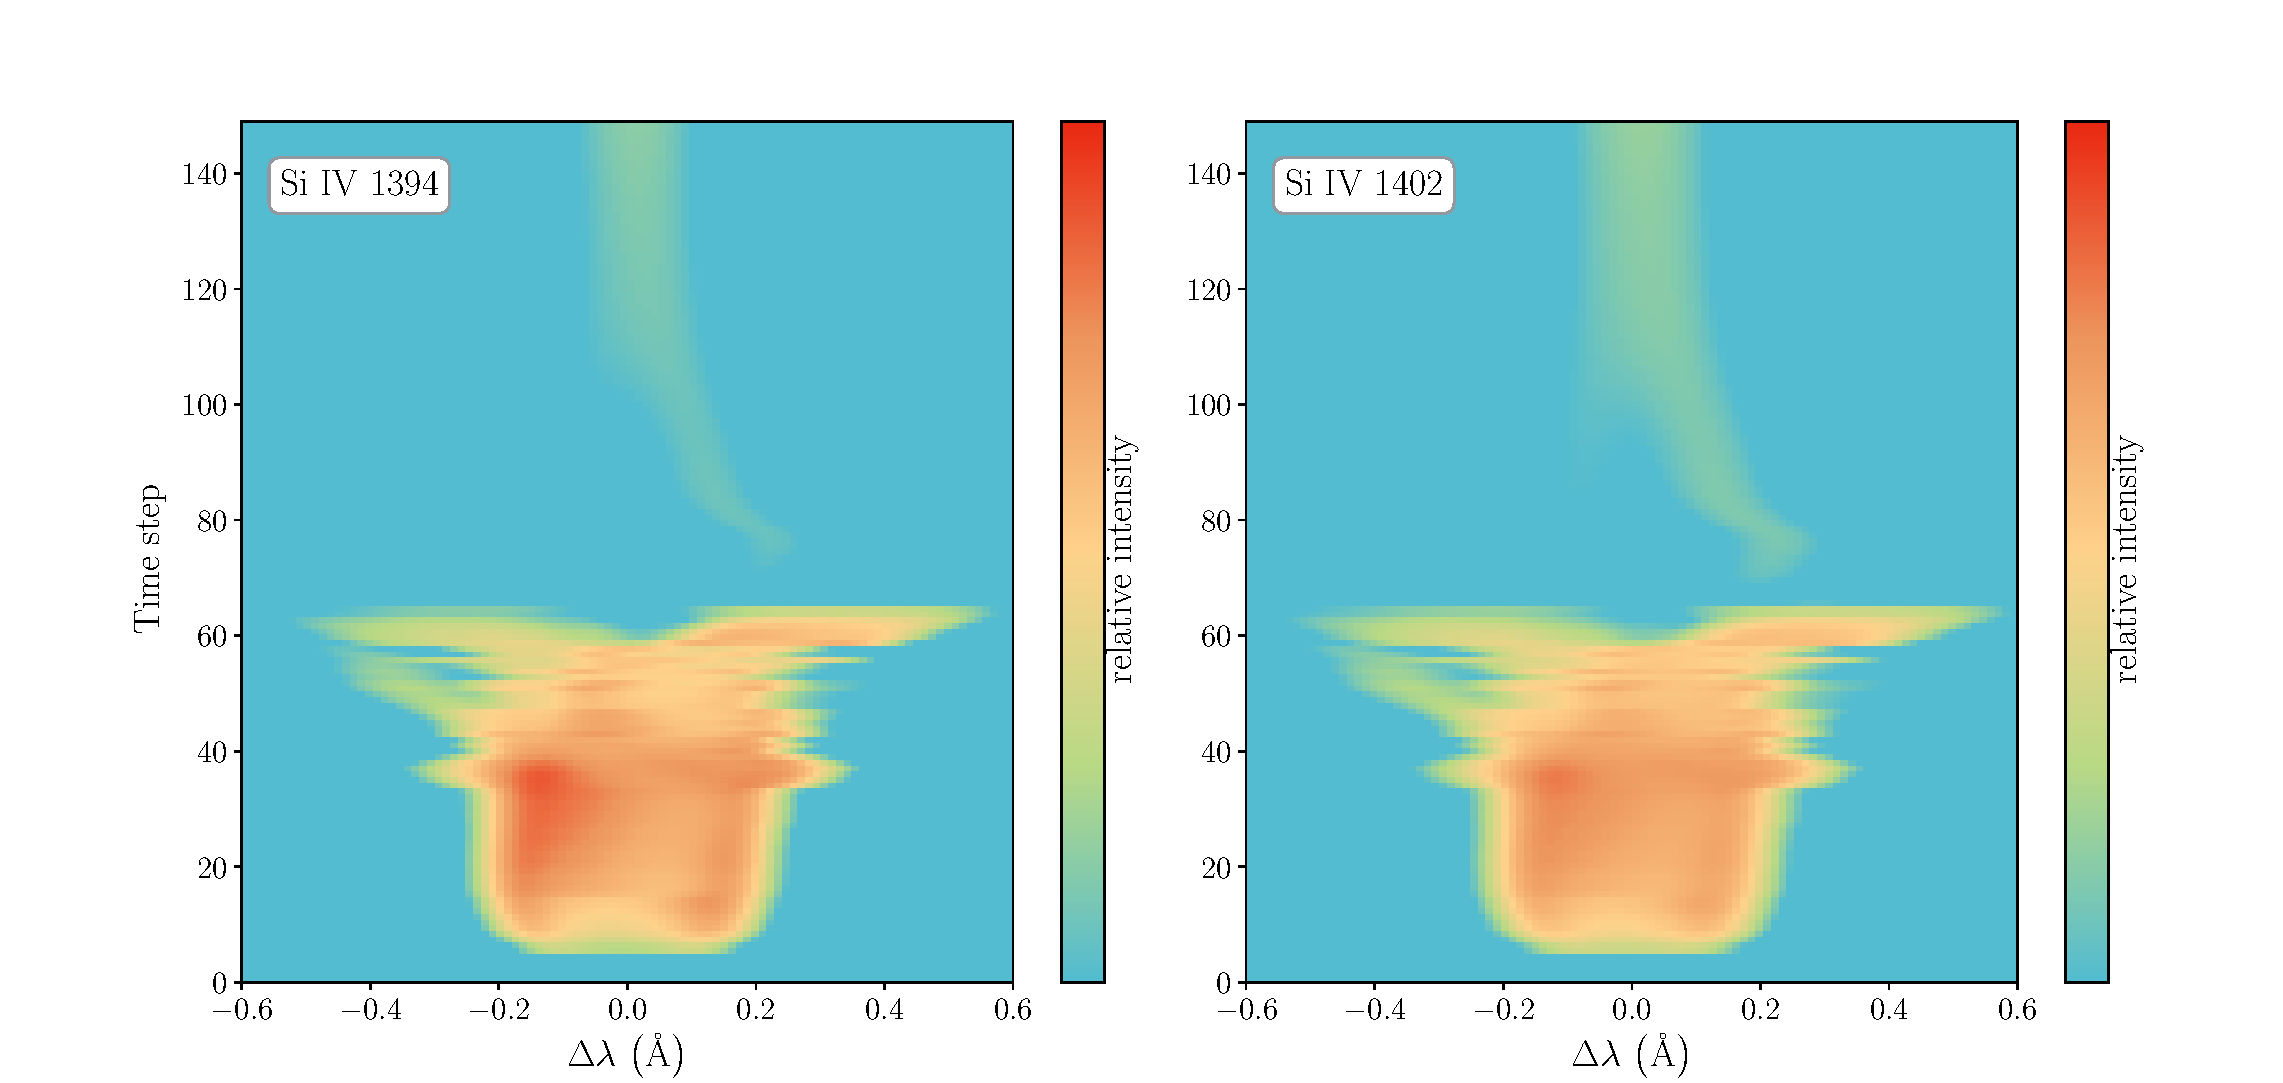
\includegraphics[width=\textwidth]{figs/5F11_spectra_imshow_Si}
	\caption{Si \textsc{iv}双重线强度随时间演化图,横坐标为波长,纵坐标为不同时刻,颜色代表该波长和时刻下的辐射强度。}
	\label{fig:3.8}
\end{figure}
我们在这一部分讨论Si \textsc{iv}双重线在光学厚辐射代码中合成光谱轮廓随时间演化的相关内容。近期有研究表明,Si \textsc{iv}双重线在耀斑爆发过程中可能是光学厚的\parencites{Kerr2019}。其中Si \textsc{iv}原子模型来源于基于RH的光学厚反演代码STiC\parencites{Rodriguez2016,Rodriguez2019},其原子模型是与RH代码相互兼容的。整个Si \textsc{iv}原子模型包含了5个Si III的能级和4个Si \textsc{iv}的能级(其中两个是Si \textsc{iv}的基态和连续态)。图~\ref{fig:3.8}展示了Si \textsc{iv}双重线内的辐射强度随着时间的演化,某些时刻的特征谱线轮廓展示在图~\ref{fig:3.9}中。
\begin{figure}
	\centering
	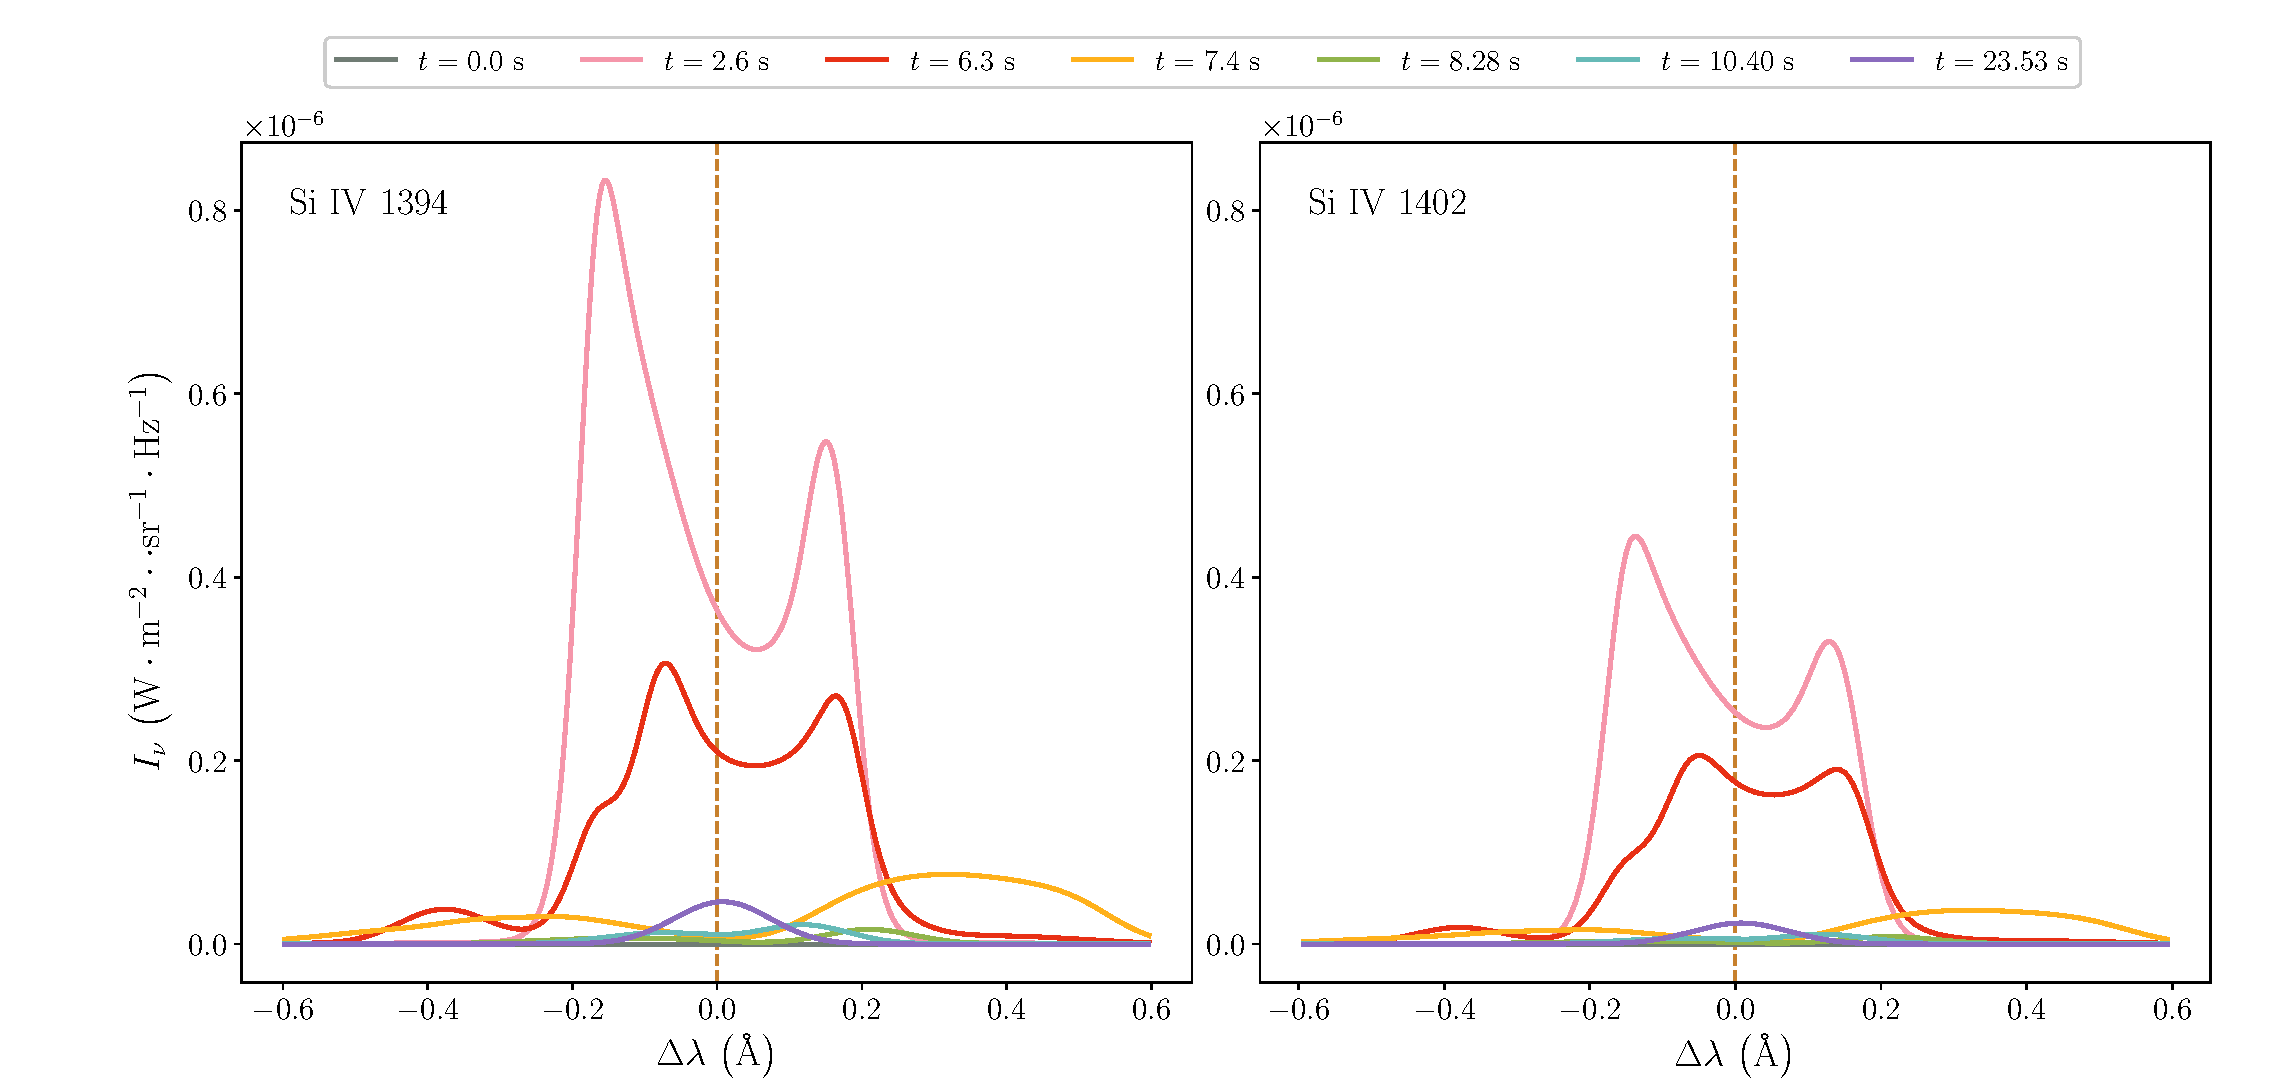
\includegraphics[width=\textwidth]{figs/5F11_spectra_line_Si}
	\caption{和图~\ref{fig:3.1}中时刻相近大气中计算得到的Si \textsc{iv}双重线谱线轮廓。}
	\label{fig:3.9}
\end{figure}

与C \textsc{ii}线相比,Si \textsc{iv}双重线的计算并没有出现数值问题。我们在计算时使用了一个比较大的微湍动速度$15\ \mathrm{km\  s^{-1}}$以再现Si \textsc{iv}形成在过渡区中的真实情况。具体的谱线演化与C \textsc{ii}线类似,一开始$t=2.6$ s线心反转的谱线的蓝侧峰不断增强,但是整个谱线的平分线速度(\textit{bisector velocity})并不大。随着加热的继续进行Si \textsc{iv}谱线的强度并没有继续增强,但是出现了一个小的蓝移分量($t=6.3$ s)。在$t=7.4$ s时,由于剧烈的色球凝聚和蒸发过程,谱线出现了一个很大的红移分量和一个比较小的蓝移分量。随着物质下流速度的逐渐减小,$t=8.28$ s和$t=10.40$ s时仅能看到一个相对较弱的红移分量。直到$t=23.53$ s时这个红移分量又逐渐回到静止波长位置,且辐射强度有一定程度的增强。



另外一个值得注意的变化是Si \textsc{iv}双重线的强度比,在光学薄极限下,两线强度比应该为2:1,在光学厚极限下则为1:1。从图~\ref{fig:3.9}中我们可以明显的看到,在模拟开始的时刻$t=2.6$ s和靠近结束的$23.53$ s,两线强度比似乎能够比较好地满足2:1的关系,而在某些时刻(如$t=6.3$ s),谱线的强度明显不符合这个关系,预示着此时的谱线的形成可能是光学厚的。为了能够更好地理解这两条谱线强度比在整个模拟过程中的演化,我们计算了两条线的积分强度随着时间的变化关系(见图~\ref{fig:3.10})。在耀斑发生一开始,两谱线比尚能维持在$1.8$左右,而当物质下流速度较大时($t>5$ s),两条谱线的强度比逐渐变小,当物质下流速度开始减小时($t\sim 7$ s),两条线的强度比又重新上升,一度到达2.0附近,但又很快重新下降,最后随着大气逐渐变得平静,两条谱线的强度比又重新向2.0移动。整个5F11模型中两线强度比的变化和\textcites{Kerr2019}中的结果相近,且进一步说明了在耀斑带上复杂的大气结构中,Si \textsc{iv}线可能形成在光学厚的环境中。

\begin{figure}
	\centering
	\includegraphics[width=0.6\textwidth]{figs/5F11_spectra_line_Si_ratio}
	\caption{Si \textsc{iv}双重线积分强度比随时间演化图。}
	\label{fig:3.10}
\end{figure}

同样的,基于Mg \textsc{ii}谱线在$t=23.53$ s与IRIS卫星观测比较匹配的结果,我们试图比较此时刻IRIS观测的Si \textsc{iv}双重线轮廓与合成光谱轮廓之间的关系。可以看到在IRIS观测中的谱线轮廓有着非常明显的红翼不对称性和一定的红移,而在$t=23.53$ s的Si \textsc{iv}则呈现出对称和几乎没有Doppler频移的特点。同时和C \textsc{ii}有着比较好拟合的$t=13.0$ s时的Si \textsc{iv}合成谱线则表现出一个蓝翼增强,和整个谱线轮廓更加不相符合。
\begin{figure}
	\centering
	\includegraphics[width=0.7\textwidth]{figs/5F11_IRIS_SiIV}
	\caption{RH合成光谱中$t=13.0$ s和$t=23.53$ s时Si \textsc{iv}谱线轮廓与IRIS观测比较。由于IRIS此次观测没有Si \textsc{iv} 1393 \mbox{\AA}线的数据,我们仅比较了红翼的这条Si \textsc{iv}线,竖线代表了其静止波长。IRIS观测经过辐射定标之后被乘以了一个5的因子使的其强度能够与合成光谱相比较。}
\end{figure}
\section{谱线形成分析}\label{sec:3.7}
最后我们通过\ref{sec:1.2.2}节中描述的贡献函数方法来分析一些和观测拟合比较好的谱线轮廓的形成高度和对应一些大气参数。首先是拟合比较好的Mg \textsc{ii}线,首先我们在图~\ref{fig:3.11}中对比了一个有较明显线心反转和一个几乎没有线心反转的谱线轮廓。可以看到合成光谱中Mg \textsc{ii}线心是否出现线心反转是和线心形成高度的电子密度密切相关的。

图~\ref{fig:3.11}中左侧的线心反转谱线形成在$t=10.0$ s处,由于色球层已经被压缩,整个线心形成高度只有大约$142$ m。由于形成于平均速度下流为$\sim36\ \mathrm{km\  s^{-1}}$的区域,谱线有明显的红移。线心形成位置温度约为$\sim 1.5\times10^4$ K,电子密度约为$5.84\times10^{14}\ \mathrm{cm^{-3}}$。由于电子密度相对较小,原函数$S_\nu$在线心形成高度上和Planck函数$B_\nu$有较大差距,因此线心处的辐射不足,产生了线心反转。而右侧的位于$t=27.56$ s的谱线轮廓,由于此时线心形成位置的体速度只有$\sim 5\ \mathrm{km \  s^{-1}}$,因此此时的谱线红移较小。与之前线心反转的谱线相比,此时的谱线形成高度的平均电子密度较大,达到了$\sim 7.8\times10^{14}\ \mathrm{cm^{-3}}$。较高的电子密度保证了线心形成在近似LTE的位置,有足够的辐射强度产生单发射峰。

由此我们也可以简单解释为什么图~\ref{fig:3.3.5}中较小$\mu = 0.2$下的Mg \textsc{ii}谱线轮廓会更宽且有更加明显的线心反转。由于$\mu$较小,说明视线方向与平面平行层大气的法线方向夹角越大,此时我们看到的是与$\mu=0.77$相比从大气更高部分发出的光子。那里的线翼形成高度电子密度更大,线心部分源函数$S_\nu$与Planck函数$B_\nu$的脱耦更明显,因此谱线更宽但线心反转更明显。


\begin{figure}[htbp]
	\begin{minipage}[t]{0.5\linewidth}
	\centering
	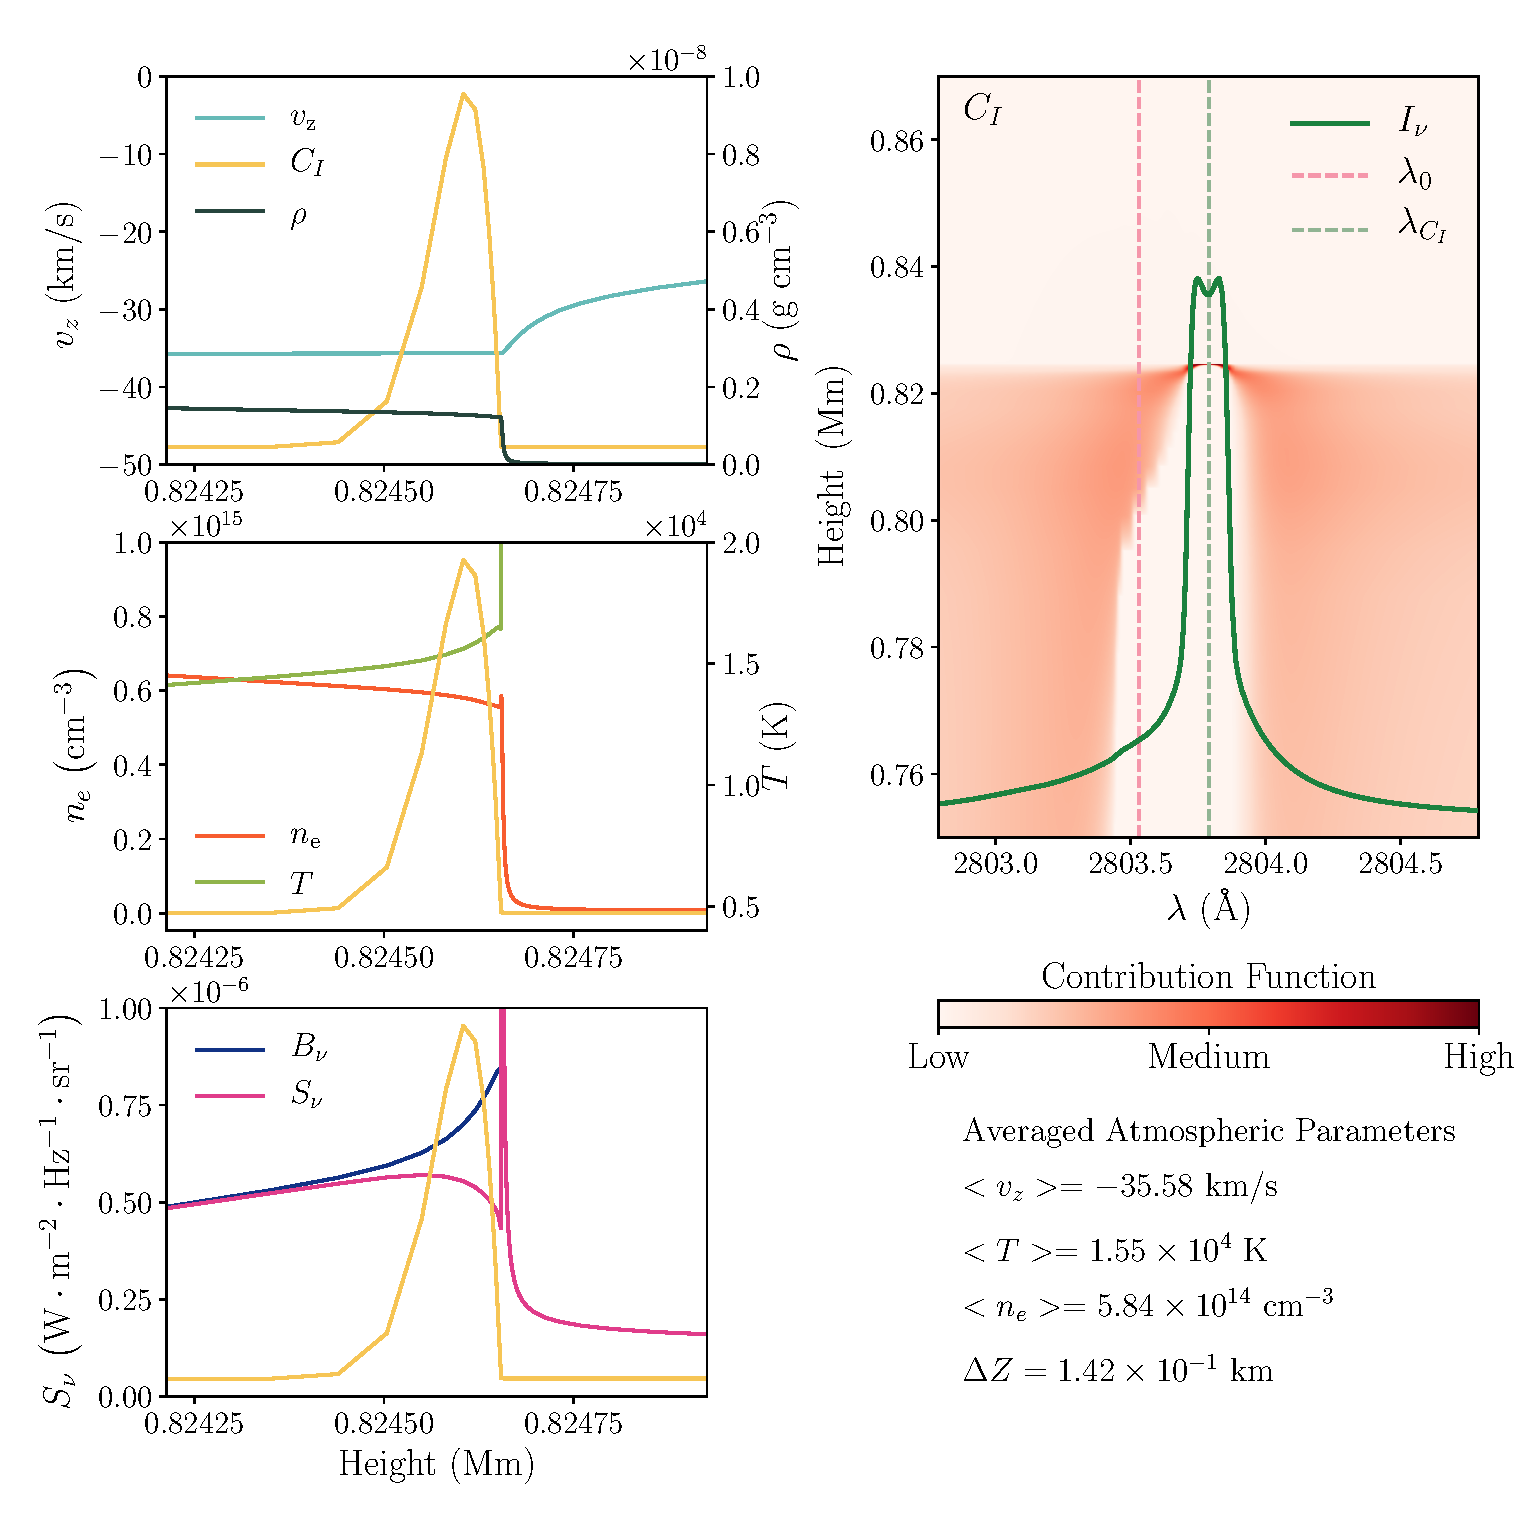
\includegraphics[width=\linewidth]{figs/ctb_5F11_88_lc}
	\end{minipage}%
	\hfill
	\begin{minipage}[t]{0.5\linewidth}
	\centering
	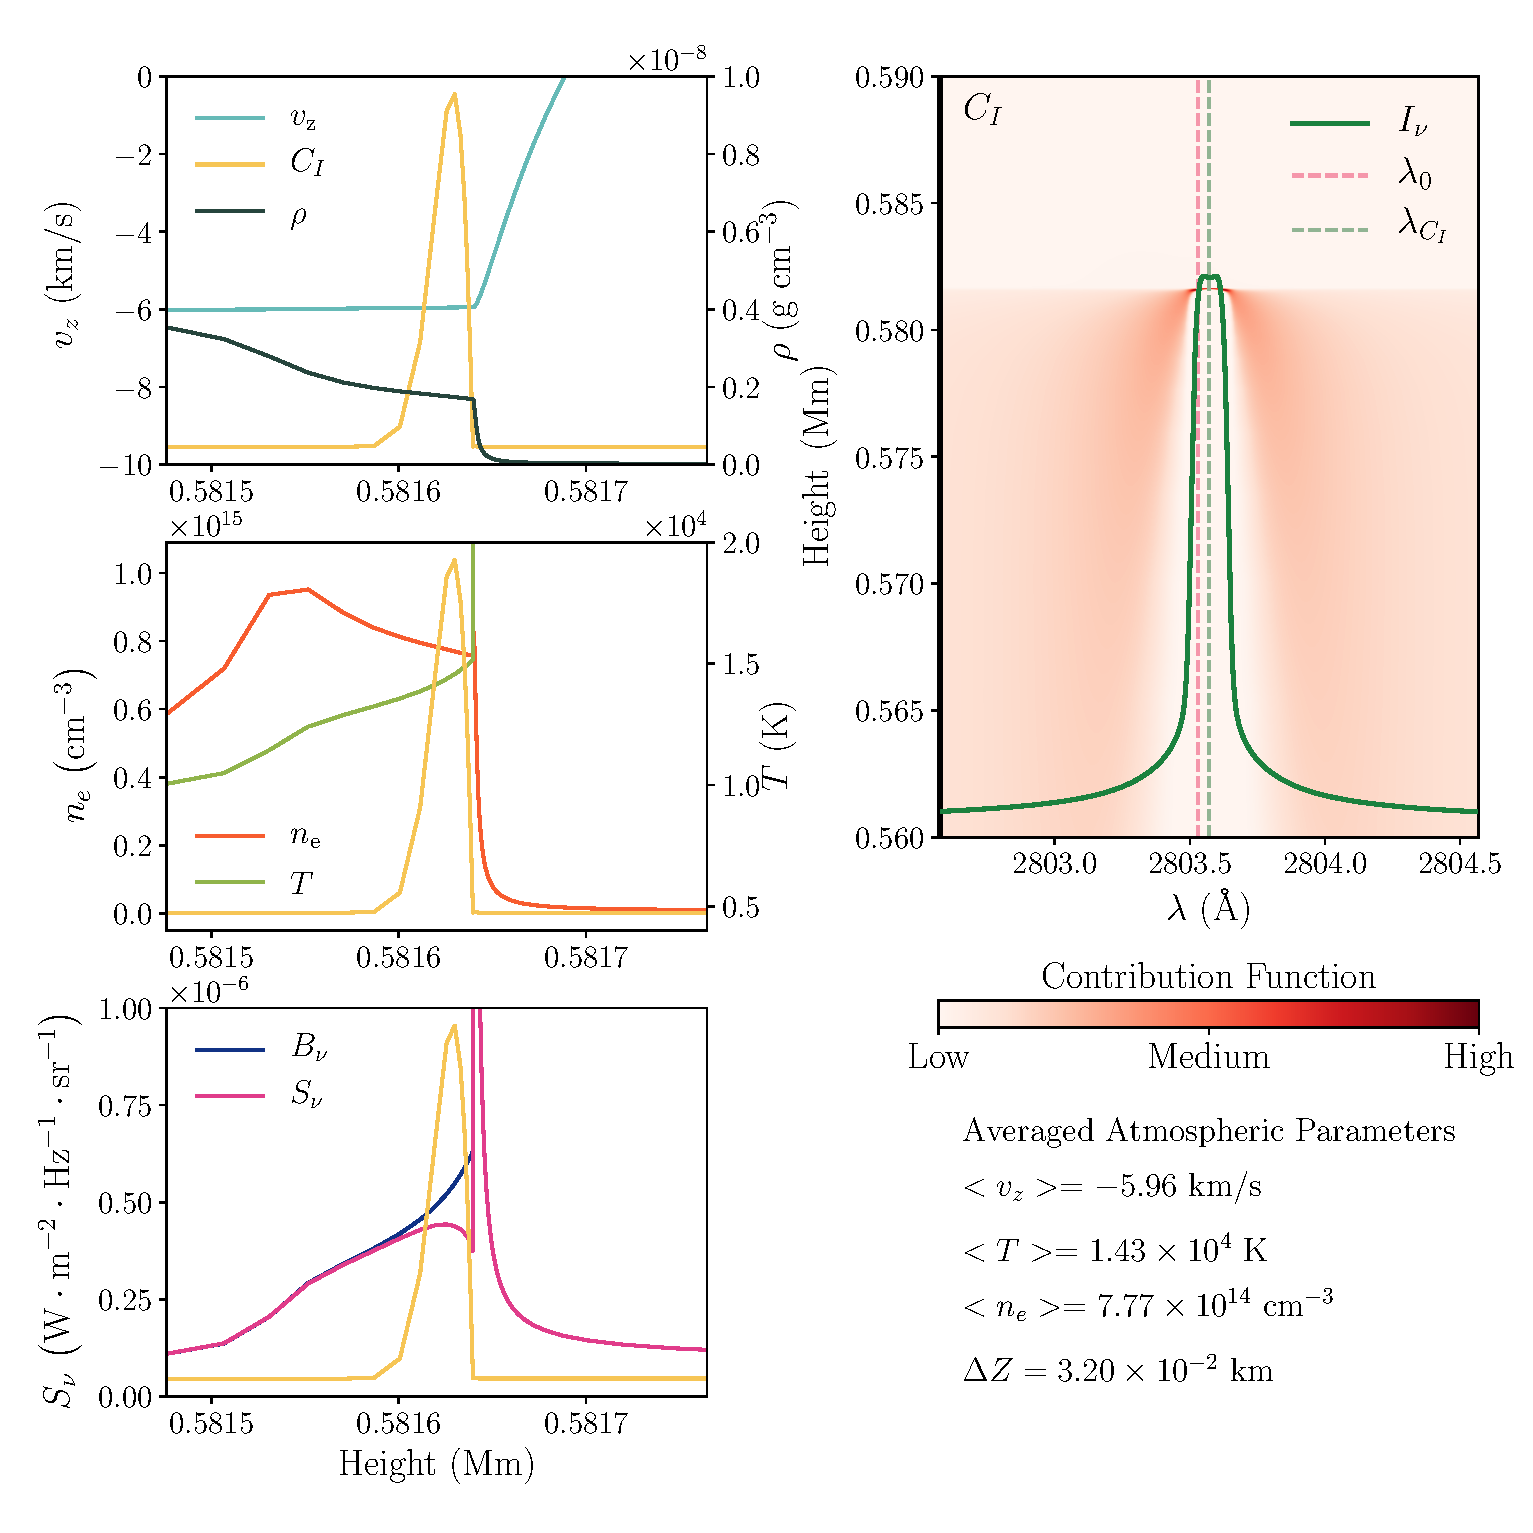
\includegraphics[width=\linewidth]{figs/ctb_5F11_250_lc}
	\end{minipage}
	\caption{左:$t=10$ s时Mg \textsc{ii} h线的贡献函数分析;右:$t=27.56$ s时Mg \textsc{ii} h线的贡献函数分析。每个图中的内容是:左上——一维速度、密度、$\lambda_c$处贡献函数随高度分布;左中——温度和电子密度随高度分布;左下——源函数和Planck函数随高度分布;右上——谱线轮廓与贡献函数在频率和波长上的分布;右下——以贡献函数作为权重函数对形成区域内的大气参数的加权平均。}
	\label{fig:3.11}
\end{figure}

\begin{figure}[htbp]
	\begin{minipage}[t]{0.5\linewidth}
	\centering
	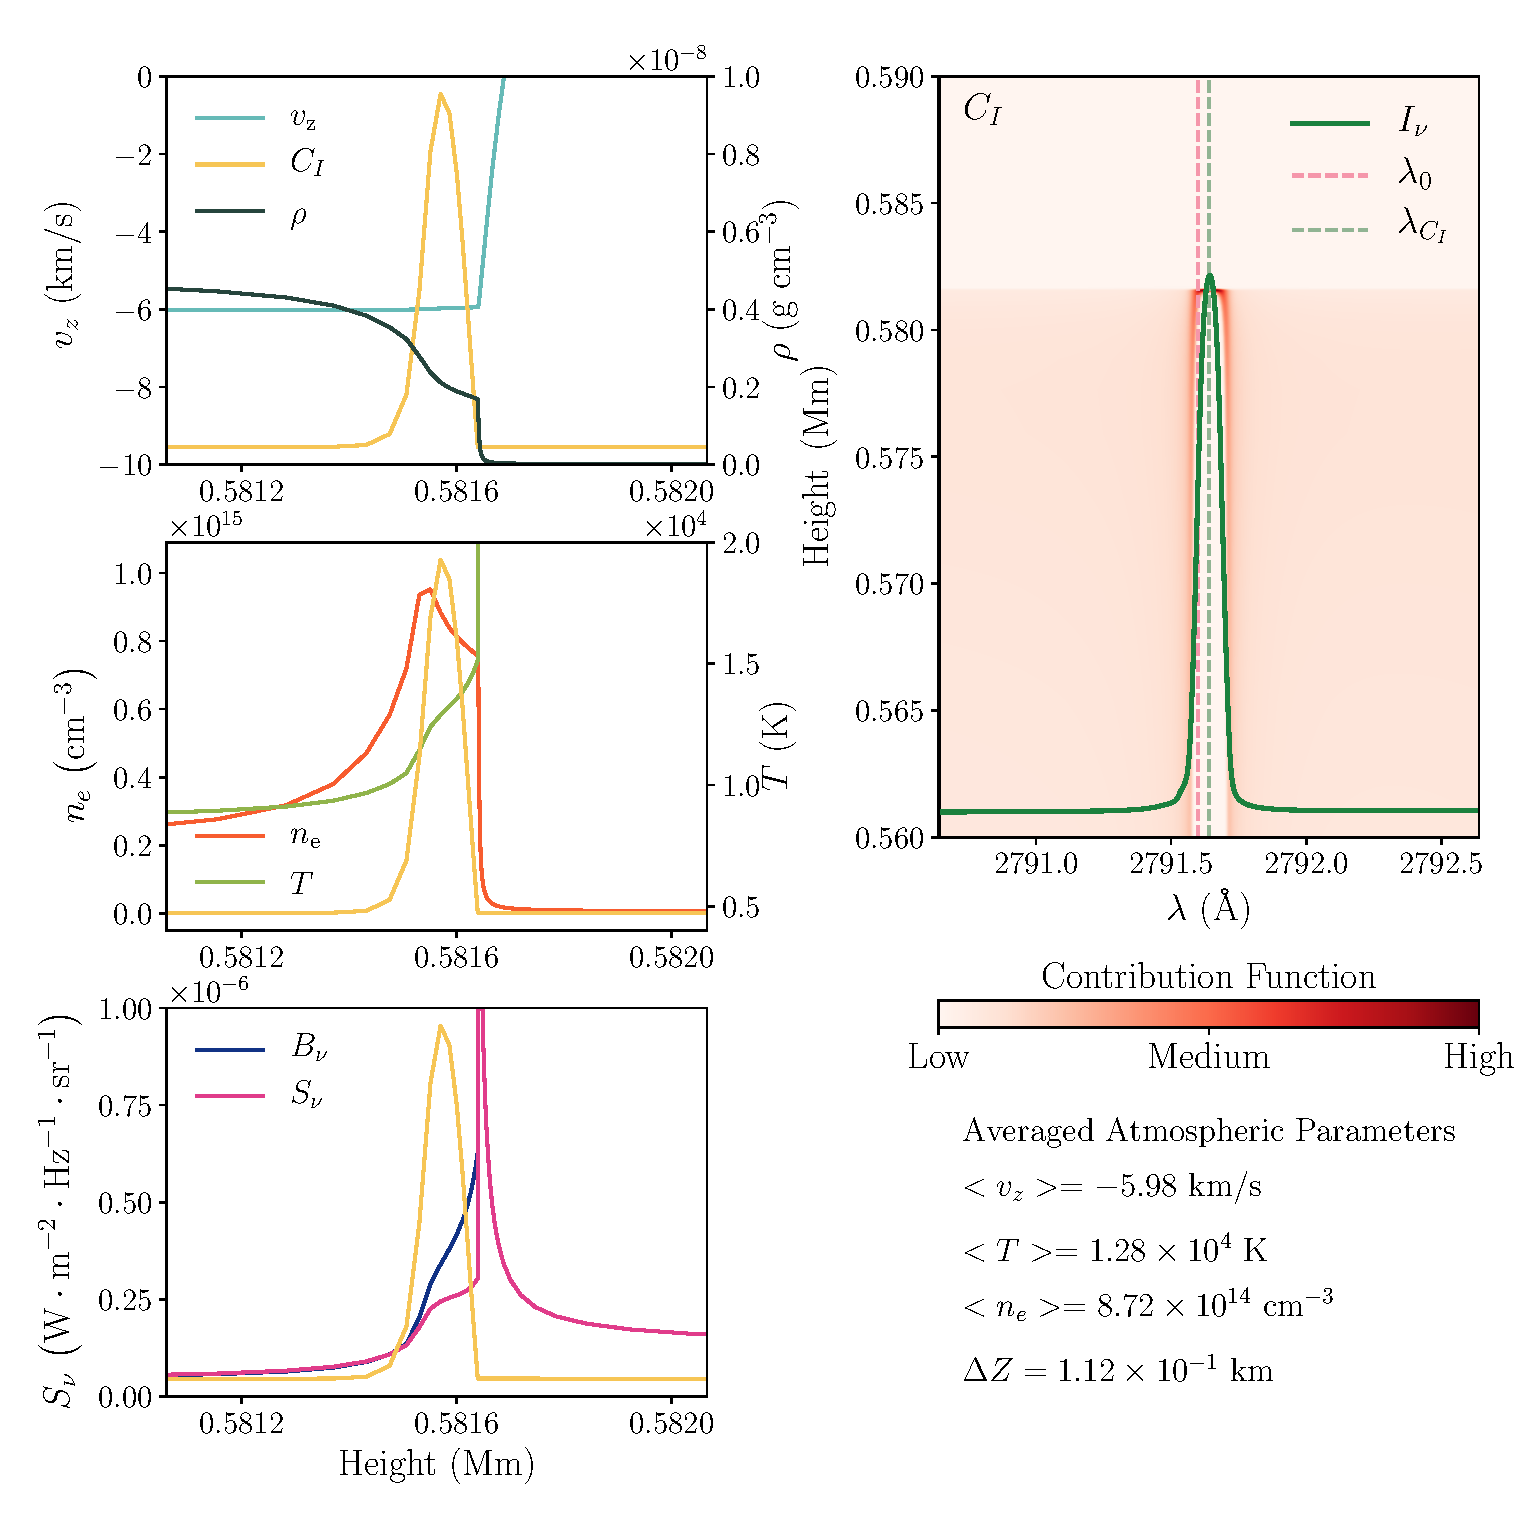
\includegraphics[width=\linewidth]{figs/ctb_5F11_250_lc_2}
	\end{minipage}%
	\hfill
	\begin{minipage}[t]{0.5\linewidth}
	\centering
	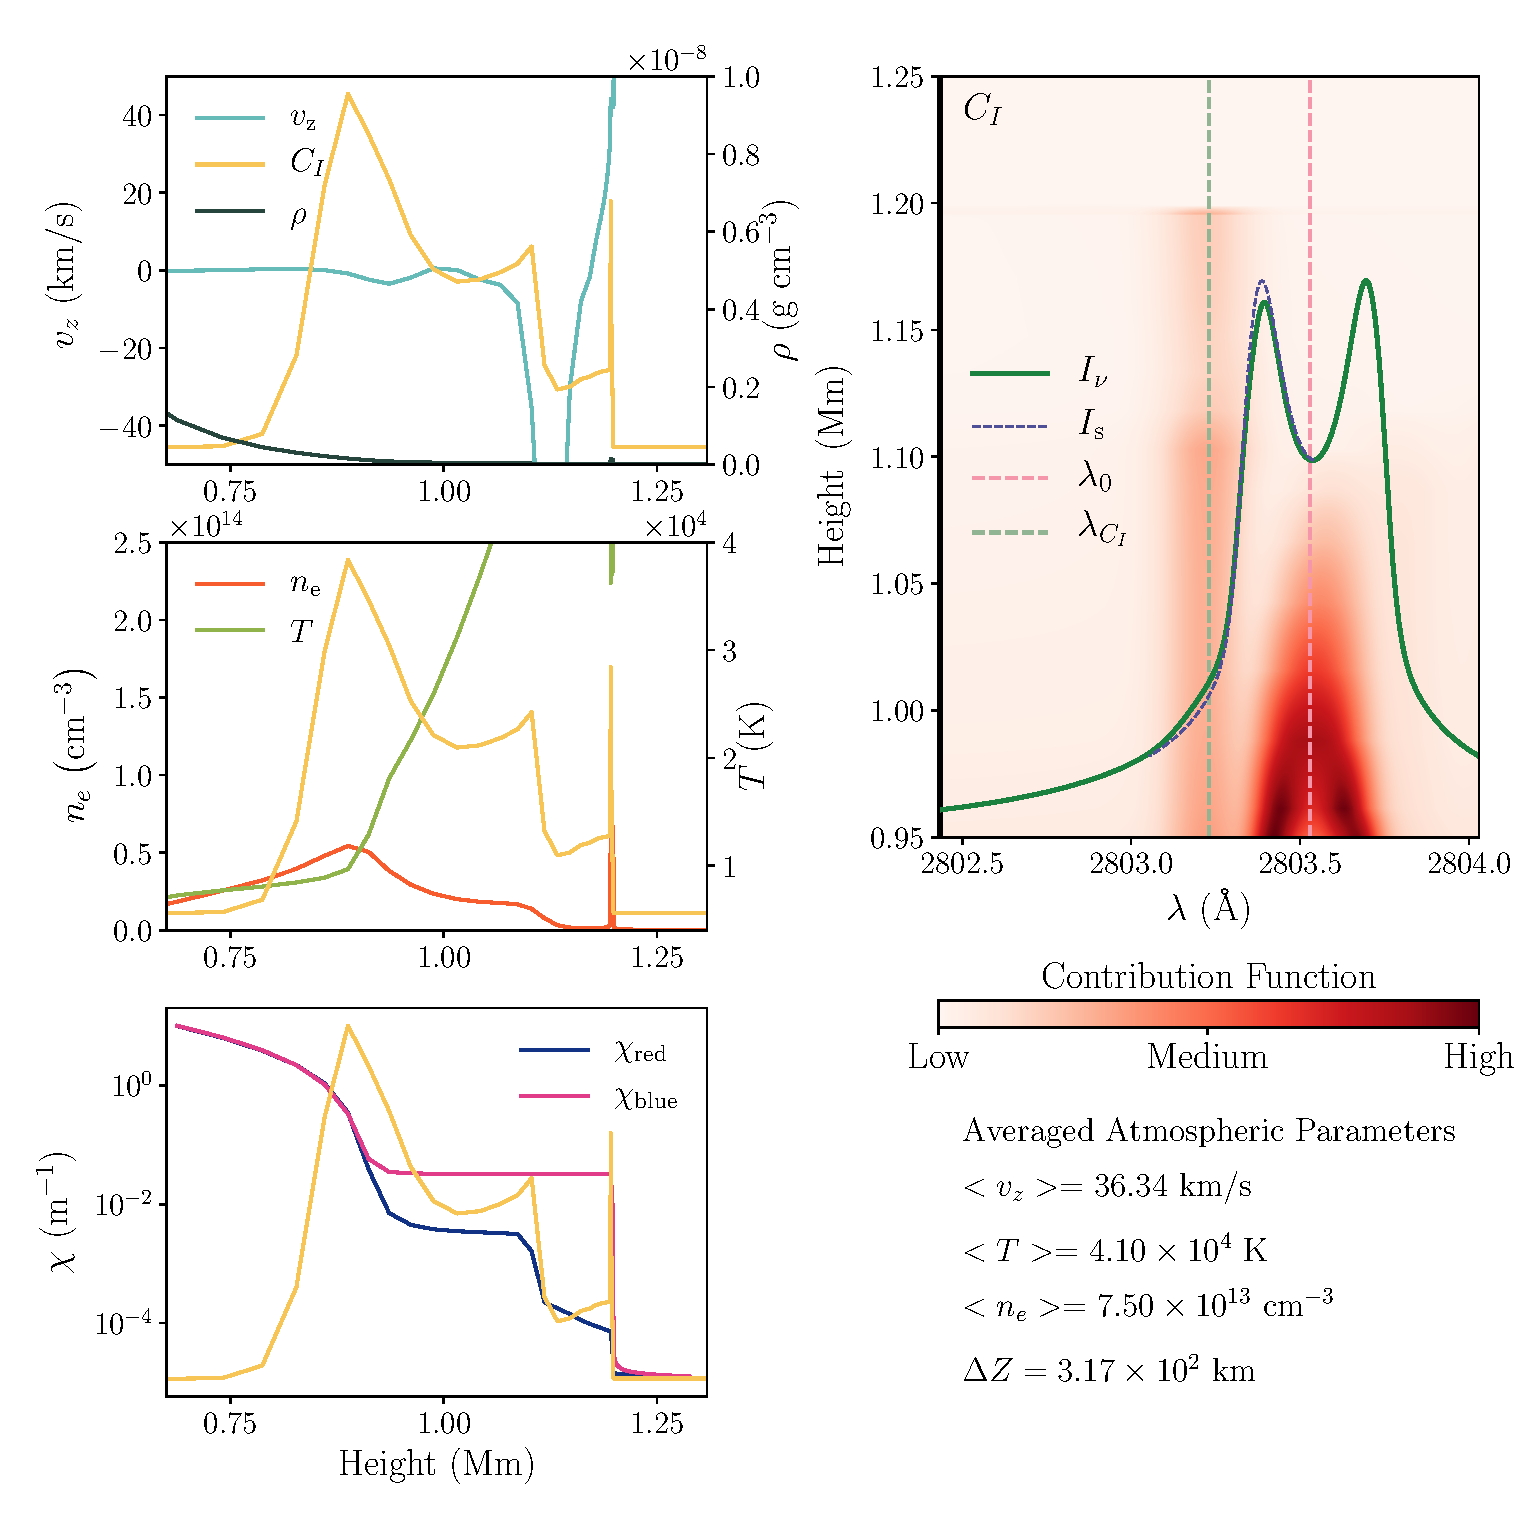
\includegraphics[width=\linewidth]{figs/ctb_5F11_44}
	\end{minipage}
	\caption{左:$t=27.56$ s时Mg \textsc{ii} 2791 \mbox{\AA}线的贡献函数分析;右:$t=5.30$ s时在RH+SB$\times$30中计算的Mg \textsc{ii} h线的贡献函数分析。其平均大气参数是在上流的冷物质部分求的平均。}
	\label{fig:3.12}
\end{figure}

图~\ref{fig:3.12}左栏展示了和图~\ref{fig:3.11}中非线心反转Mg \textsc{ii} h线同时的Mg \textsc{ii} 2791 \mbox{\AA}线,通过对其线心形成高度的分析,我们发现其生成在和Mg \textsc{ii} h线非常相近的高度上。这也解释了为什么我们在\ref{sec:3.4}节中对Mg \textsc{ii} h和k线线心形成高度的微湍动速度进行进一步调整时,Mg \textsc{ii}三重线也会剧烈致宽。

图~\ref{fig:3.12}右栏展示了$t=5.30$ s一个具有微弱蓝翼不对称性的Mg \textsc{ii} h谱线轮廓,我们使用了RH+SB$\times$30代码来计算谱线轮廓使其线翼辐射能够和实际观测相比。对蓝翼增强位置的贡献函数分析表明,这一增强来自于一个冷的物质上流提高了这一波长位置的不透明度。这团上流物质的特征温度约为$\sim4\times10^4$ K,速度约为$\sim 36\ \mathrm{km\  s^{-1}}$,电子密度约为$7.5\times10^{13}\ \mathrm{cm^{-3}}$。

\begin{figure}[htbp]
	\begin{minipage}[t]{0.5\linewidth}
	\centering
	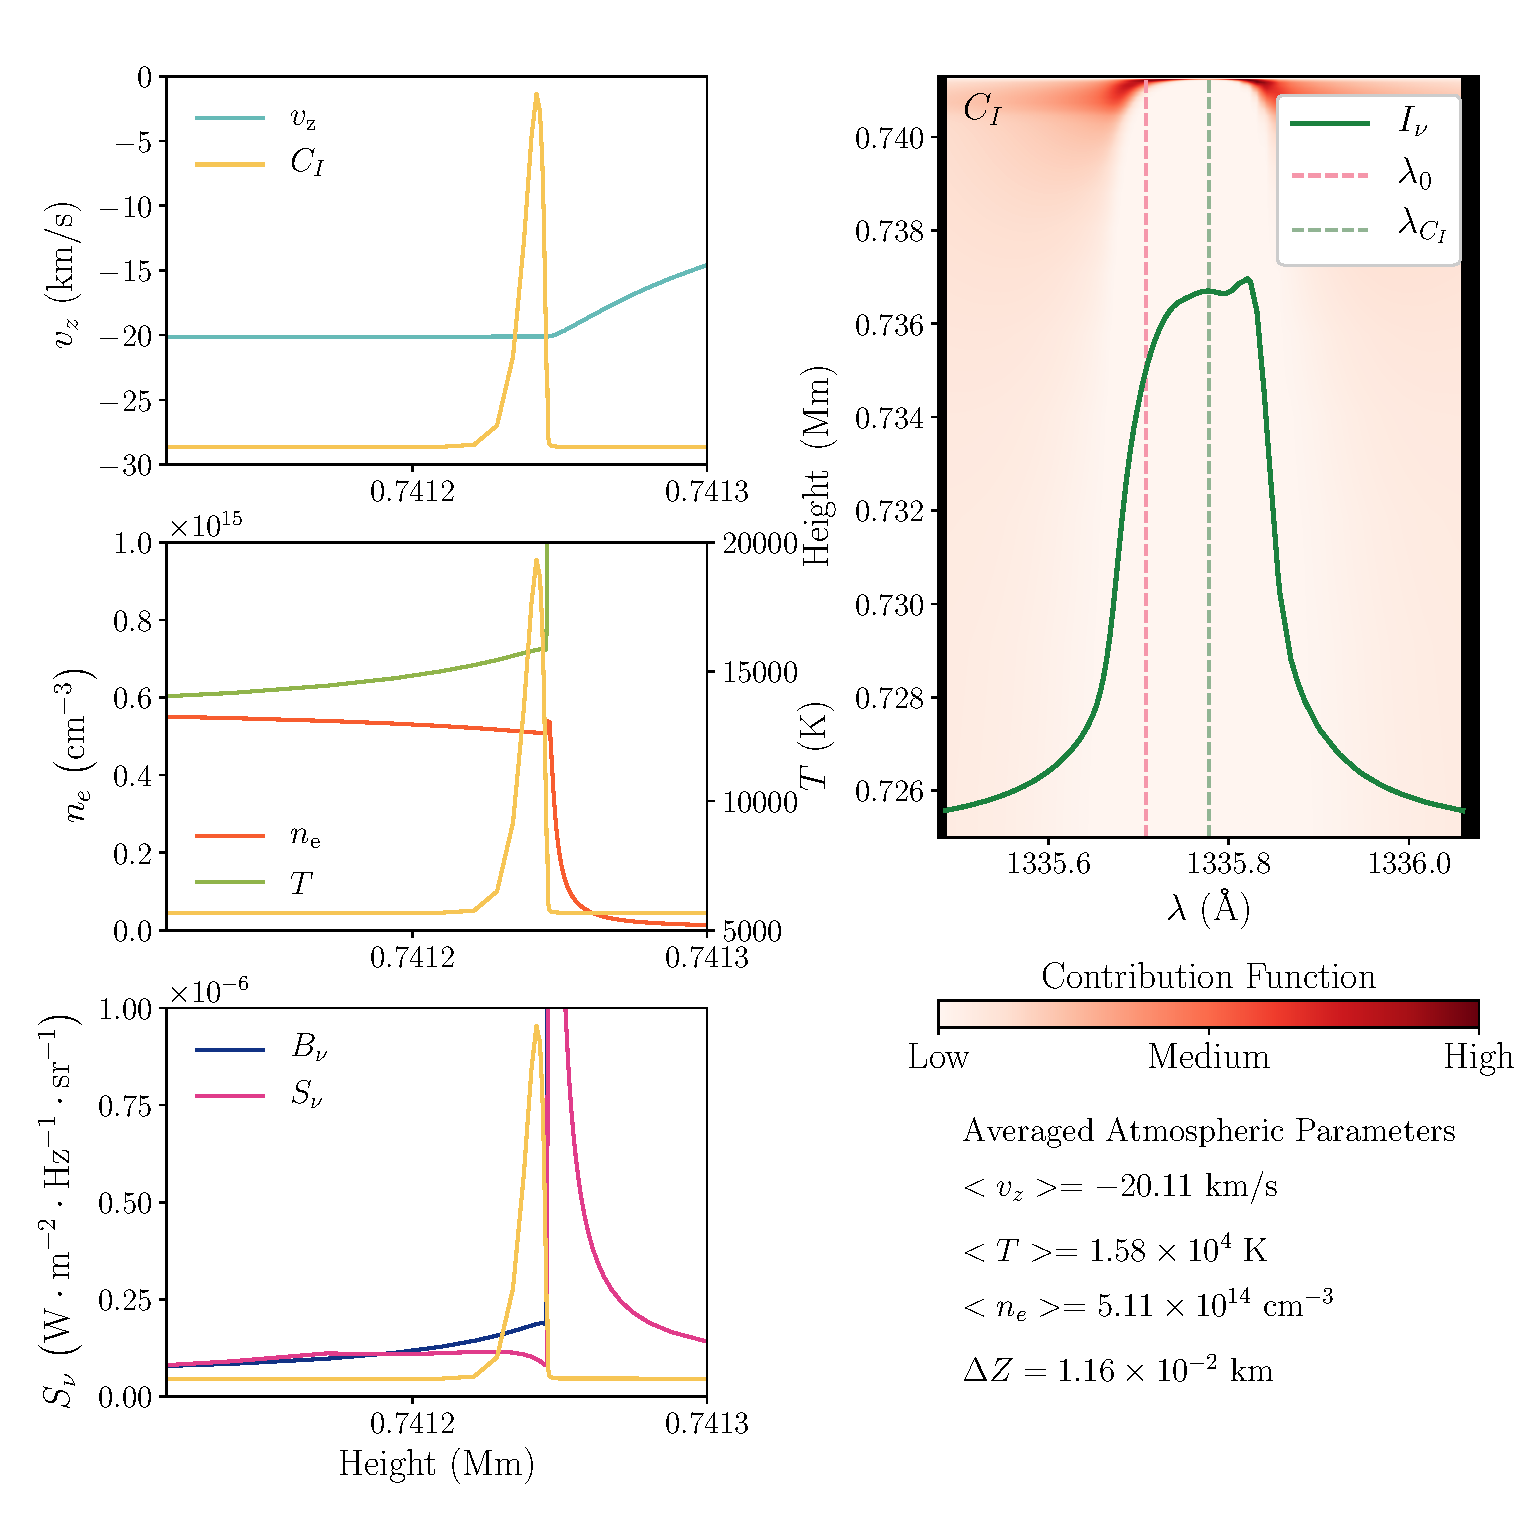
\includegraphics[width=\linewidth]{figs/ctb_5F11_112_CII}
	\end{minipage}%
	\hfill
	\begin{minipage}[t]{0.5\linewidth}
	\centering
	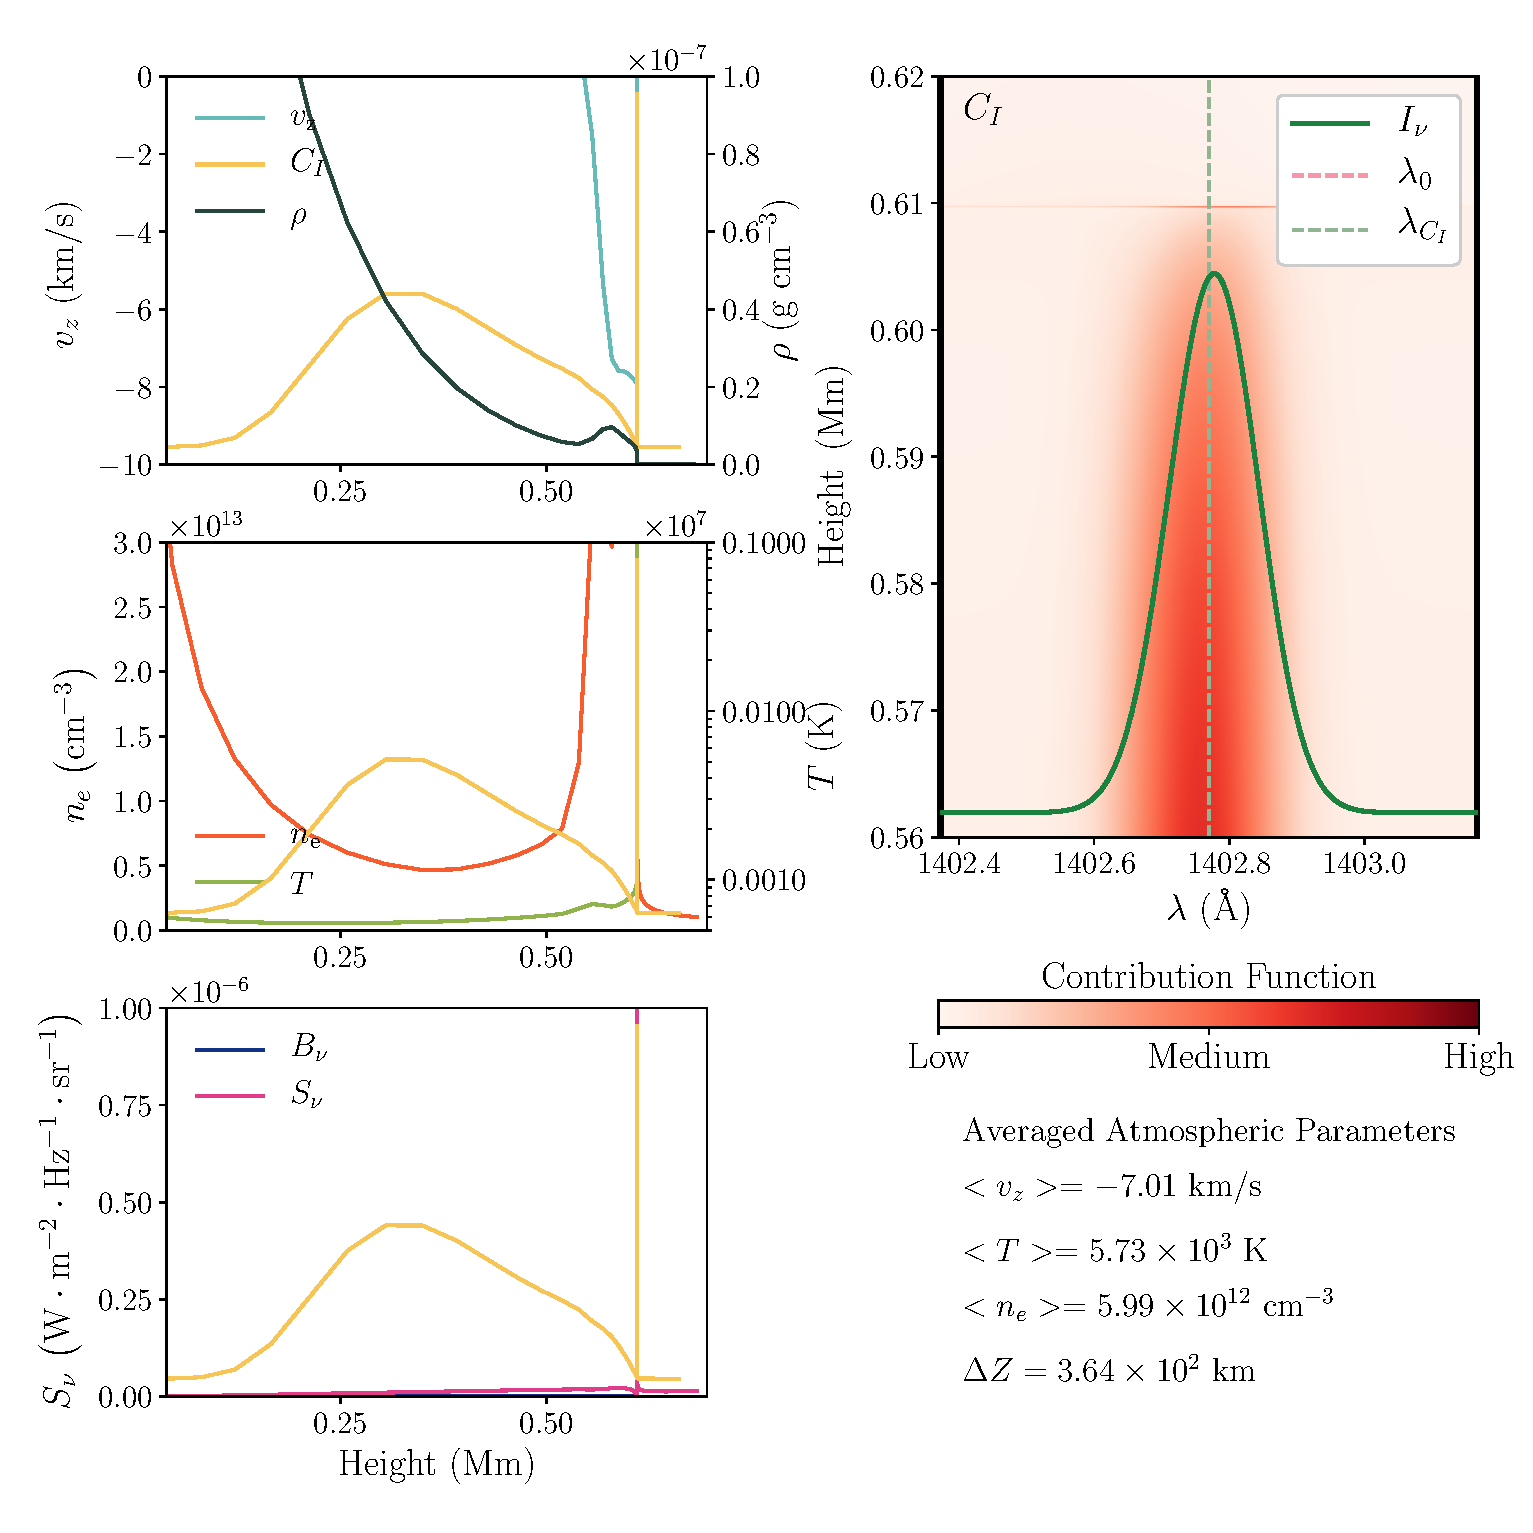
\includegraphics[width=\linewidth]{figs/ctb_5F11_SiIV_210}
	\end{minipage}
	\caption{左:$t=13.0$ s时C \textsc{ii} 1335 \mbox{\AA}线的贡献函数分析;右:$t=23.53$ s时Si \textsc{iv} 1402 \mbox{\AA}线的贡献函数分析。}
	\label{fig:3.13}
\end{figure}


之后我们来分析和观测符合得不太好的C \textsc{ii}和Si \textsc{iv}线。图~\ref{fig:3.13}左栏展示了$t=13.0$ s与IRIS观测在红移上拟合比较好的C \textsc{ii}线。从谱线形成高度上来看,C \textsc{ii}线的形成高度基本和Mg \textsc{ii}线重合,略高约数公里。但是C \textsc{ii}线线心形成区域受色球压缩的影响更强,其线心形成范围只有$\sim 11$ m,紧贴在过渡区下面。形成高度上的温度约为$\sim1.6\times10^4$ K,电子密度约为$\sim 5.1 \times 10^{14}\ \mathrm{cm^{-3}}$。

图~\ref{fig:3.13}右栏中展示的是Si \textsc{iv}线在$t=23.53$ s时谱线轮廓和贡献函数分析,值得注意的是这里Si \textsc{iv}线心除了一个位于过渡区的明显贡献之外,还存在着大量来自色球的贡献,因此说明此时的合成光谱是不太可靠的。我们将在之后\ref{sec:3.8}节中的讨论中分析为什么RH代码在此时计算Si \textsc{iv}谱线轮廓出现了问题。
\section{He \textsc{i} 10830 \mbox{\AA}线的Stokes参数变化}
在最后我们想尝试通过RH代码支持的计算整个谱线的Stokes参数的辐射转移的功能。He \textsc{i} 10830 \mbox{\AA}三重线是位于近红外的三条重要发射线,他们的空气波长为10829.09 \mbox{\AA},10830.250 \mbox{\AA}和10830.34 \mbox{\AA},真空波长为10832.06 \mbox{\AA},10833.22 \mbox{\AA}和10833.31 \mbox{\AA}。分别来自于能级$1s2p\ ^3P_0-1s2s\ ^3S_1$,$1s2p\ ^3P_1-1s2s\ ^3S_1$和$1s2p\ ^3P_2-1s2s\ ^3S_1$的跃迁。它们一般形成在高色球区域,离日冕约$\sim 2$ Mm的位置\parencites{Avrett1994,Chaouche2012}。目前对其的形成高度和谱线轮廓等尚未有较为详细的辐射流体力学模拟研究,但在具体观测中已经被广泛地用于色球磁场的测量中。特别是在耀斑带上,近期\textcites{Libbrecht2019}利用10830线和He \textsc{i} $D_3$线研究了耀斑带上的磁场强度,认为耀斑带上有大约$\sim 2500$ G的磁场。而\textcites{Anan2018}对一个C级耀斑耀斑带上的He \textsc{i} 10830 \mbox{\AA}的Stokes参数进行了观测,并利用弱场近似得到了耀斑带上大约有$\sim 1000$ G左右的磁场。

目前尚没有能够对He \textsc{i} 10830线进行高空间和光谱分辨率观测的望远镜和仪器。但随着下一代太阳望远镜-拥有4 m主镜的Daniel K. Inouye太阳望远镜(\textit{DKIST}, \cites{DKIST2014})的建成,其所搭载的衍射极限近红外分光偏振计(\textit{Diffraction Limited Near Infrared Spectropolarimeter, DL-NRISP}: \cites{DKIST2007})将使用He \textsc{i} 10830 \mbox{\AA}作为用于测量太阳色球磁场的重要谱线之一。整个DL-NRISP将以前所未有的空间分辨率(最高至0.5个角秒)和光谱分辨率($R\sim 250000$)同时测量Stokes $I$,$Q$,$U$,$V$四个参数。届时,He \textsc{i} 10830 \mbox{\AA}肯定会在太阳色球磁场测量中发挥相当重要的作用。

基于这样的考虑,我在RH的大气输入模型中手动插入了一个$B_z = 500$ G的磁场,然后计算He \textsc{i} 10830 \mbox{\AA}谱线内的I,Q,U,V四个参数的辐射转移。图~\ref{fig:3.14}展示了整个过程中的Stokes参数随时间的演化。我们另在图~\ref{fig:3.15}中展示了一些特征时间的Stokes参数轮廓。可以看出整个He \textsc{i} 10830 \mbox{\AA}线由于形成在高色球,因此也和Mg \textsc{ii} h等线一样在电子束加热大气产生色球凝聚时产生比较大的红移,随后不断减小。谱线的线偏振度和圆偏振度都在耀斑加热相达到极值。其中代表圆偏振度的的Stokes $V/I$大约在5\%-15\%的量级,比\textcites{Anan2018}对C级耀斑的观测结果稍大。
\begin{figure}
	\centering
	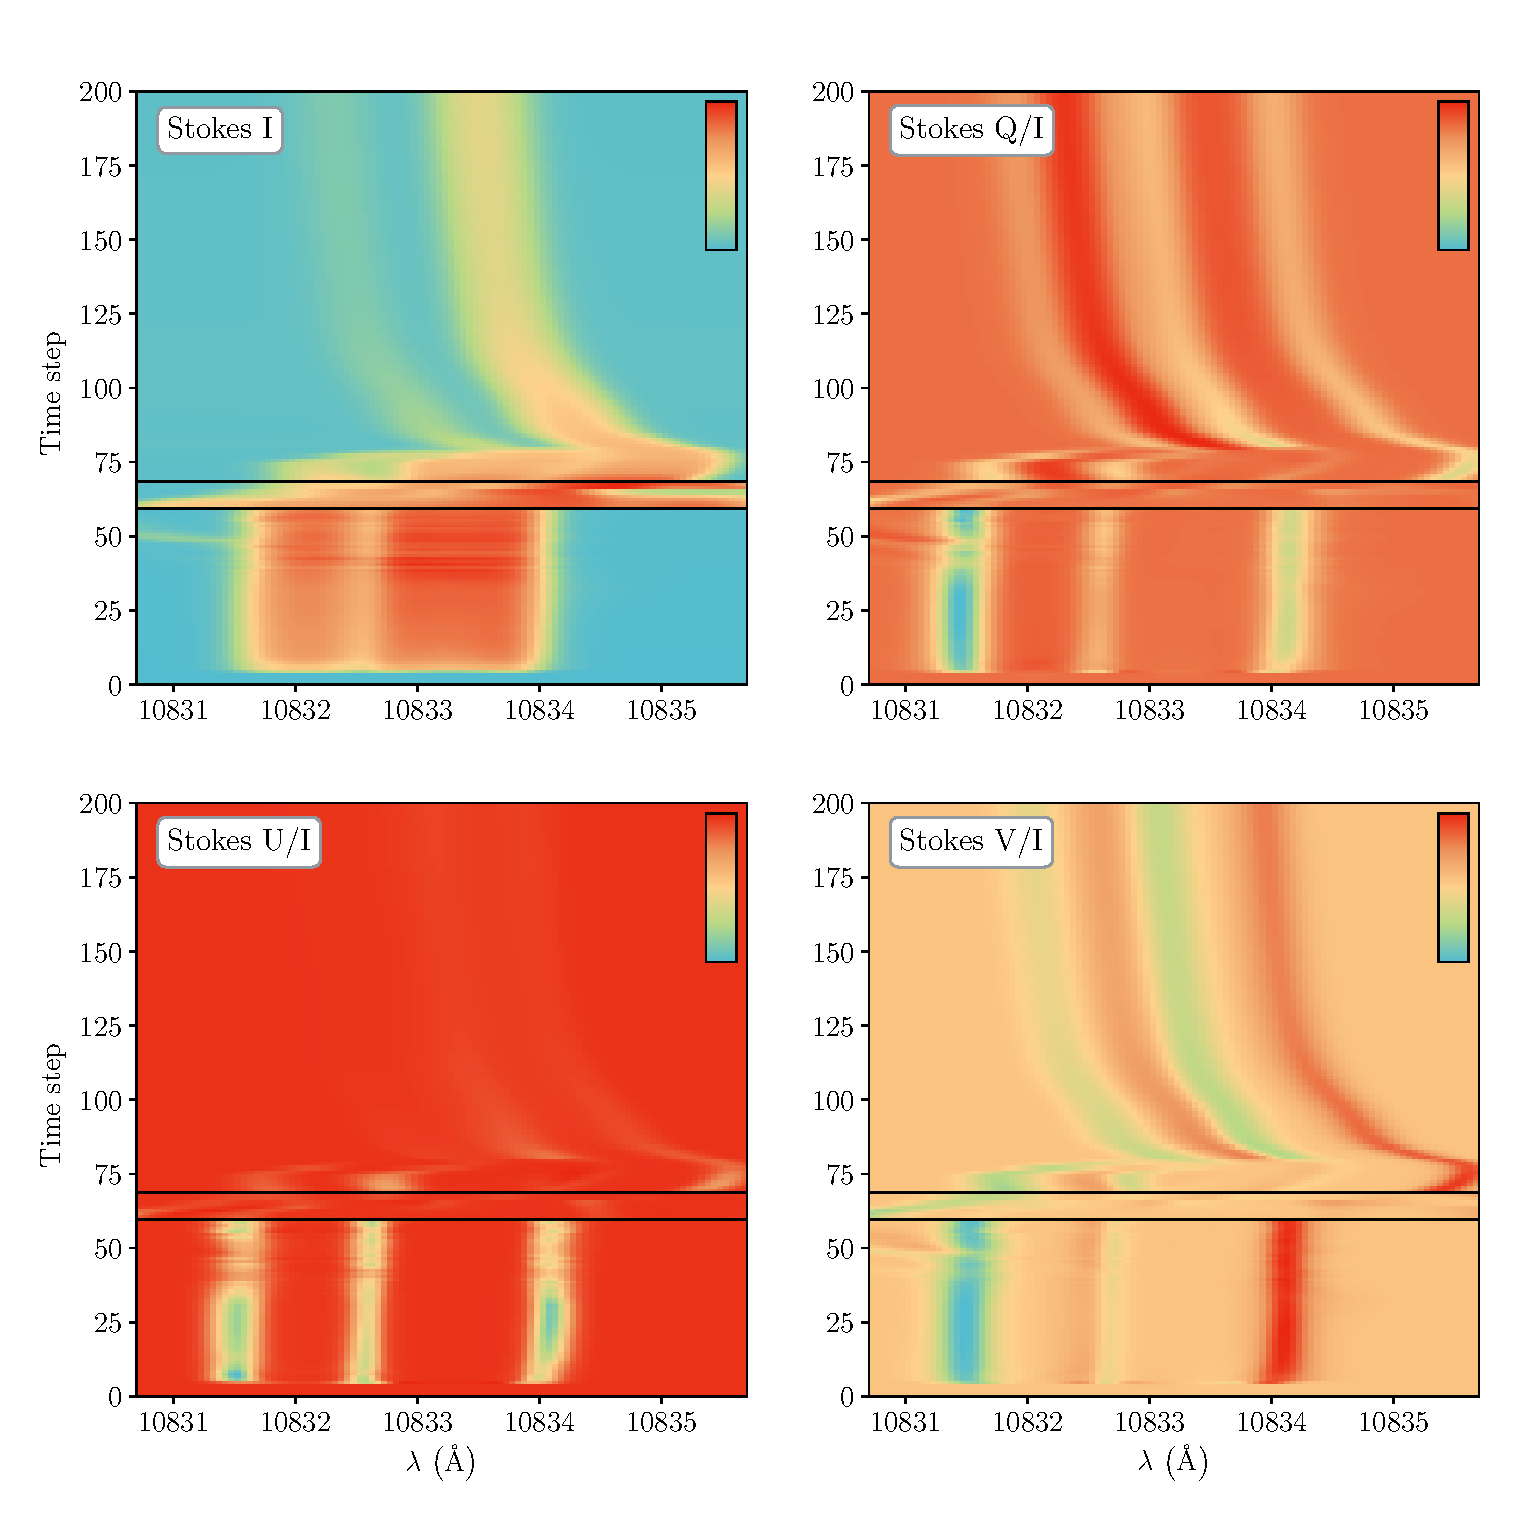
\includegraphics[width=0.6\textwidth]{figs/HeI_Stokes_imshow}
	\caption{He \textsc{i} 10830 \mbox{\AA}线Stokes参数在模拟中的演化。}
	\label{fig:3.14}
\end{figure}

\begin{figure}
	\centering
	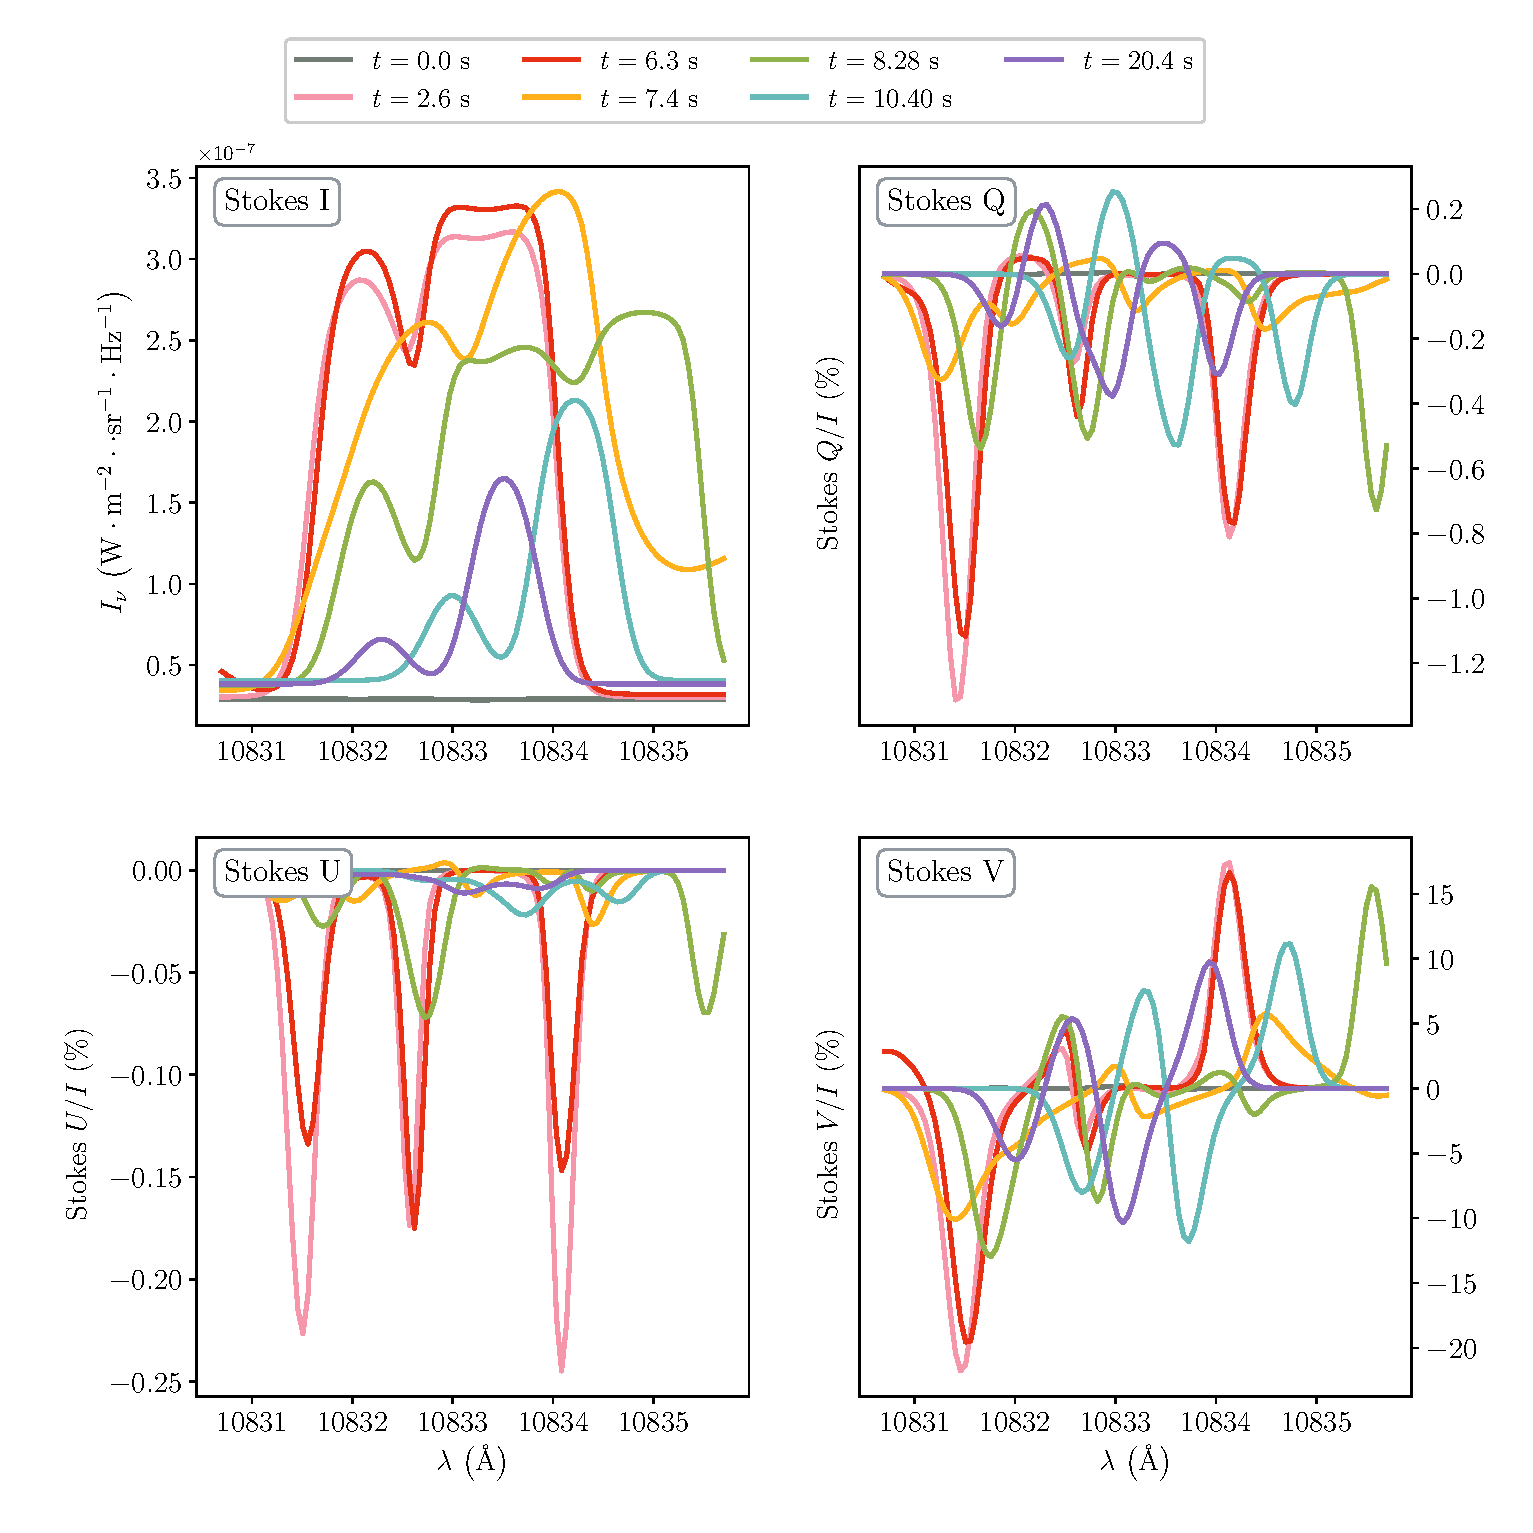
\includegraphics[width=0.6\textwidth]{figs/HeI_Stokes_spec}
	\caption{He \textsc{i} 10830 \mbox{\AA}线Stokes参数某些特定时刻的形状。}
	\label{fig:3.15}
\end{figure}
\section{讨论}\label{sec:3.8}
首先我们来关注如何解释Mg \textsc{ii}和C \textsc{ii}等谱线需要通过继续增大Stark宽度才能较好地再现耀斑带上谱线急剧致宽的谱线轮廓的问题。关于这一点,我们从目前RADYN和RH代码的一些缺陷出发,探讨模拟中可能忽略的一些重要效应:
\begin{enumerate}
	\item 非热电子的影响:显然入射的非热电子同样会对Mg \textsc{ii}的离子能级产生影响\parencites{Hawley2007},由于它们的能量往往更大,产生的Stark致宽效应也往往更强烈。尽管在我们的模型中这些入射的非热电子的密度$\sim10^{10}\ \mathrm{cm^{-3}}$往往远小于当地的热电子密度,但是它们应该仍然能够在热化的过程中和周围的其他电子相互作用,而这些局地的电子再与Mg \textsc{ii}离子能级产生相互作用。此外,这些非热电子对Mg \textsc{ii}粒子的非热激发和电离作用也会改变Mg \textsc{ii}离子的能级粒子数,从而影响谱线轮廓形状。以上和非热电子有关的因素都是目前的计算中所没有考虑的,我们的Stark致宽只考虑了周围热电子的影响,且没有考虑这些非热电子的非平衡电离效应。
	\item 三维辐射转移效应:\textcites{Leenaarts2013a}指出三维辐射转移效应对Mg \textsc{ii}谱线线心的形成至关重要。目前尚没有对耀斑过程中的色球谱线进行完全自洽大气内的三维辐射转移计算的工作,因此我们猜测其可能也会对谱线的致宽做出贡献。
	\item 磁场:模拟中没有考虑磁场对大气动力学演化的影响。尽管之前有相关研究表明Mg \textsc{ii}对磁场是有一定敏感性的\parencites{Ballester2016},但我们基于RH代码的计算表明,在1000 G左右的磁场并不能对辐射强度,即Stokes $I$参数产生重要的影响。
	\item 电子密度:\textcites{Rubio2017}通过手动增加大气中的电子密度至$\sim 10^{15}\ \mathrm{cm}^{-3}$来获得非线心反转的谱线,而这一电子密度的高峰已经在我们的自洽大气中找到。但是在她们的参数模拟中,这个电子密度的高峰在高度的分布上更广,甚至达到了线翼的形成位置。如果我们能够在自洽大气的线翼形成位置也能形成$10^{14}\ \mathrm{cm^{-3}}$以上的电子密度,是有可能进一步增大Stark致宽的。
\end{enumerate}

关于Mg \textsc{ii}谱线剧烈致宽的另外一个解释来自于\textcites{Rubio2017},她们认为多个尚未在观测上得以分辨的$200\ \mathrm{km\  s^{-1}}$以上的宏观物质对流叠加有能够产生剧烈致宽的谱线。在我们的模拟中,在$t=7.35$ s左右由于在一个一维大气中同时存在速度上流和下流,的确获得了剧烈加宽的Mg \textsc{ii} h和k线(见图~\ref{fig:3.4})。但是由于物质下流与致密的中低层色球大气的相互作用,此时刻附近的约为$100\ \mathrm{km \  s^{-1}}$的物质下流并不能在模拟上持续超过$1$ s的时间。因此不能产生超过1 \mbox{\AA}以上的远红翼的辐射增强。\textcites{Rubio2017}中假想存在的这样的高速度的物质下流(色球凝聚)可能来自于入射非热电子的能流不均匀导致的局部大于$10^{13}\ \mathrm{erg\  cm^2\  s^{-1}}$高能流\parencites{Kowalski2015,Kowalski2018a}。

\textcites{Panos2018}通过机器学习在一系列大耀斑的耀斑带前缘提取出了带有剧烈红翼增强和部分线心反转的Mg \textsc{ii} h和k谱线轮廓。在整个耀斑带前缘扫过这些区域后,出现的是常见的单峰、剧烈致宽的Mg \textsc{ii} h和k谱线轮廓。整个谱线的演化过程和我们5F11模型中的Mg \textsc{ii}演化过程比较类似。在我们的模拟过程中的$t=7-10$ s间先产生了有较大红移的Mg \textsc{ii} h和k线,而后这些谱线的红移逐渐减小,并且因为色球被高度压缩而产生的电子密度增加(至$\sim 8\times 10^{14}\ \mathrm{cm^{-3}}$)而出现了非线心反转的谱线。

最近\textcites{Tei2018}发现了Mg \textsc{ii}线在耀斑一开始发生时的蓝移(蓝翼增强)现象。在此之后,Mg \textsc{ii}谱线才出现常见的红翼不对称性。她们认为这个蓝翼的增强来自于一个上流的冷物质湍,并用一个简单的云模型计算了Mg \textsc{ii}谱线的辐射转移。她们发现对于当这团物质温度为$T=10^4$ K且上流速度为$v_z\sim 40\ \mathrm{km \  s^{-1}}$时能够非常好的拟合观测到的谱线。正如图~\ref{fig:3.13}右栏所示的,我们的5F11模拟中也同样发现具有蓝翼增强的谱线情况,且出现在整个谱线轮廓的剧烈红移发生之前。在我们的模拟中这团冷物质的温度大约为$4\times 10^4$ K,速度约为$\sim 36\ \mathrm{km \  s^{-1}}$。由于在模拟中的这团物质温度较高,因此在C \textsc{ii}和Si \textsc{iv}线上也能看到蓝翼增强的分量,这与她们的观测有一定的差异。同时我们的这团冷物质的存在时间只有$\sim 1-2$ s,而\textcites{Tei2018}则发现了整个谱线蓝移过程持续了数十秒。尽管如此,我们的模拟还是支持她们对Mg \textsc{ii}谱线在耀斑带开始增亮时出现蓝翼增强的解释。

\begin{figure}
	\centering
	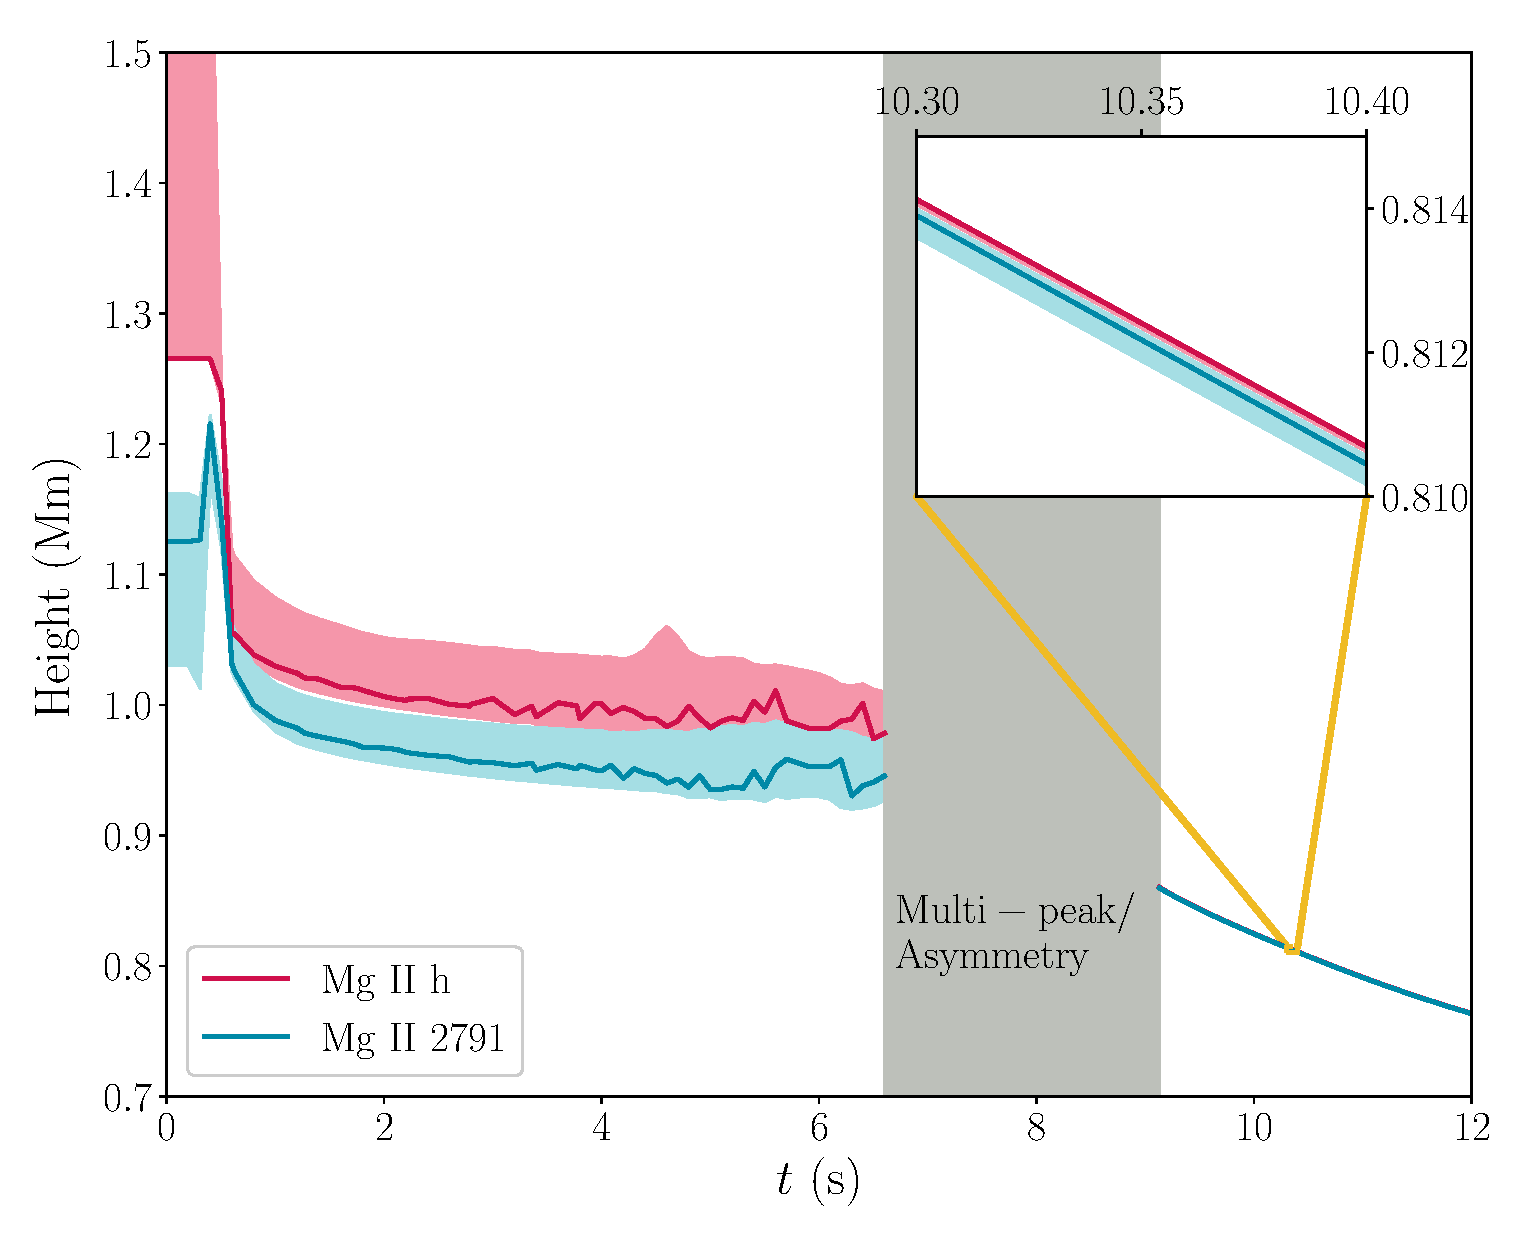
\includegraphics[width=0.6\textwidth]{figs/formation_height}
	\caption{5F11模型中Mg \textsc{ii} k与2791三重线线心形成位置随着时间的演化图。我们通过积累贡献函数$C_I'=0.16$与$C_I'=0.84$来确定整个谱线的形成区间。其中青色代表Mg \textsc{ii} 2791 \mbox{\AA}线,红色代表Mg \textsc{ii} k线。灰色部分代表由于谱线的过于不对称和多峰结构导致无法确定线心位置的时刻。}
	\label{fig:3.16}
\end{figure}
另外值得一提的是我们发现在模拟后期Mg \textsc{ii} h和k线出现非线心反转谱线轮廓时,Mg \textsc{ii}三重线往往形成在同一大气高度上。之前对于宁静太阳上Mg \textsc{ii}线心的形成模拟认为它们形成在大约在过渡区下200 km\parencites{Leenaarts2013b}的高度。而Mg \textsc{ii}三重线则一般被认为形成在低色球位置\parencites{Pereira2015}。但一些在耀斑带上的一维辐射流体力学模拟表明也可以形成在较高的色球位置,约为0.83 Mm - 1.14 Mm\parencites{Rubio2017}。为了确认这一点,我们画出了Mg \textsc{ii} k线和2791三重线的形成高度随着时间的演化图(图~\ref{fig:3.16})。我们发现,一开始的大气中Mg \textsc{ii} k线心的确形成于高色球,而2791三重线线心则形成在低色球。随着时间的不断演化,$t=4$ s时两条谱线的形成区域已经相当接近且出现重叠,而当$t>10$ s后两条谱线的线心形成位置几乎是完全相同的,同样的结果同样被其他的一维辐射流体力学模拟所证实\parencites{Kerr2019}。因此我们认为当Mg \textsc{ii} h和k线出现非线心反转的谱线时,处于发射状态的Mg \textsc{ii}三重线线心很有可能形成于高色球,只能作为低色球加热的定性判据,而不应该作为定量诊断工具。

对于为什么C \textsc{ii}线和Si \textsc{iv}线难以在Mg \textsc{ii}线和观测拟合比较好的时间点再现观测到的谱线轮廓,我们也可以从目前的模拟给出一定的猜测。总的来说,我们认为目前一维辐射流体力学模拟较为欠缺的一个点是对耀斑衰变相中冷却过程的模拟。目前对这些这样的较长时间红翼不对称性的产生机制基本都集中在冷却过程上,如\textcites{Tian2015}和~\textcites{Brannon2016}认为产生需要冷却物质的下流,\textcites{Reep2016}和~\textcites{Warren2016}认为需要多个耀斑环的持续冷却。在我们的模拟中,整个色球凝聚过程随着电子束入射能流的减小而迅速减弱,不能一直产生较长时间的物质下流。因此如何在模拟上再现这样持续时间非常长的色球凝聚过程仍是亟待解决的问题。另外在我们的模拟中,C \textsc{ii}谱线的线心形成高度和Mg \textsc{ii}非常相近,但是线翼却相对高于Mg \textsc{ii}线,在实际情况中是否可能在这段区间内存在较大的速度梯度进而有足够的速度流产生大量的红翼辐射仍然存疑。

对于Si \textsc{iv}线,在之前\ref{sec:3.7}节的贡献函数分析中我们提到在模拟的合成光谱中存在来自色球温度较低的贡献。现在我们认为这些贡献实际上是来自于我们在RH代码中使用的原子模型未包含Si \textsc{i}和Si \textsc{ii}能级造成的错误。在Mg \textsc{ii}线的模拟中,我们之所以能够使用一个不包含Mg \textsc{i}原子模型的Mg \textsc{ii}离子模型去模拟谱线形成,其原因是Mg \textsc{i}和Mg \textsc{ii}都广泛存在于整个光球和中低色球的大气中,因此我们并不需要非常仔细地去考虑其电离态上的粒子数对Mg \textsc{ii}线心附近轮廓的影响。

而对于Si则恰恰相反,Si \textsc{iii}之下还有两个低电离态Si \textsc{i}和Si \textsc{ii},在低层大气中这几个电离态之间的相对粒子数对温度是相对敏感的(见图~\ref{fig:3.16})。因此如果我们在原子能级中不考虑这两个电离态,一个直接的结果是在低层大气中,本来应该大量处在Si \textsc{i}和Si \textsc{ii}能级上的原子被我们强行留在了Si \textsc{iii}和Si \textsc{iv}能级上,特别是在耀斑过程中,由于色球凝聚的出现,中低色球的密度大大增加,导致了有更多应该在Si \textsc{i}和Si \textsc{ii}能级上的原子被滞留在高能级上,产生了不应该存在Si \textsc{iv}谱线辐射。因此我们强调如果要比较好的模拟Si \textsc{iv}在太阳爆发过程中的谱线轮廓,应该使用包含Si \textsc{i}和Si \textsc{ii}两个能级的原子模型。
\begin{figure}
	\centering
	\includegraphics[width=0.5\textwidth]{figs/Si_pop}
	\caption{Si原子在不考虑电荷交换(上)和考虑电荷交换(下)的不同电离态占据数与温度之间的关系。来源:\textcites{Kerr2019}}
	\label{fig:3.16}
\end{figure}


% vim:ts=4:sw=4